% ****** Start of file apssamp.tex ******
%
%   This file is part of the APS files in the REVTeX 4.2 distribution.
%   Version 4.2a of REVTeX, December 2014
%
%   Copyright (c) 2014 The American Physical Society.
%
%   See the REVTeX 4 README file for restrictions and more information.
%
% TeX'ing this file requires that you have AMS-LaTeX 2.0 installed
% as well as the rest of the prerequisites for REVTeX 4.2
%
% See the REVTeX 4 README file
% It also requires running BibTeX. The commands are as follows:
%
%  1)  latex apssamp.tex
%  2)  bibtex apssamp
%  3)  latex apssamp.tex
%  4)  latex apssamp.tex
%
\documentclass[%
 reprint,
%superscriptaddress,
%groupedaddress,
%unsortedaddress,
%runinaddress,
%frontmatterverbose, 
%preprint,
%preprintnumbers,
%nofootinbib,
%nobibnotes,
%bibnotes,
 amsmath,amssymb,
 aps,
%pra,
%prb,
%rmp,
%prstab,
%prstper,
%floatfix,
]{revtex4-2}
\usepackage{lipsum}
\usepackage{caption}
\usepackage{subcaption}
\usepackage{siunitx}
\usepackage{gensymb}
\sisetup{separate-uncertainty=true}
\usepackage{graphicx}% Include figure files
\usepackage{dcolumn}% Align table columns on decimal point
\usepackage{bm}% bold math
\usepackage{hyperref}% add hypertext capabilities
\usepackage{xcolor}
\hypersetup{
	colorlinks,
	linkcolor={blue},
	citecolor={red},
	urlcolor={purple}
}
%\usepackage[mathlines]{lineno}% Enable numbering of text and display math
%\linenumbers\relax % Commence numbering lines

%\usepackage[showframe,%Uncomment any one of the following lines to test 
%%scale=0.7, marginratio={1:1, 2:3}, ignoreall,% default settings
%%text={7in,10in},centering,
%%margin=1.5in,
%%total={6.5in,8.75in}, top=1.2in, left=0.9in, includefoot,
%%height=10in,a5paper,hmargin={3cm,0.8in},
%]{geometry}

\begin{document}

\preprint{APS/123-QED}

\title{Study of non-linear optical properties \\using the Z-scan technique}% Force line breaks with \\
%\thanks{A footnote to the article title}%

\author{Maitrey Sharma}
% \altaffiliation[Also at ]{Physics Department, XYZ University.}%Lines break automatically or can be forced with \\
%\author{Second Author}%
% \email{Second.Author@institution.edu}
\affiliation{%
 School of Physical Sciences, National Institute of Science Education and Research, HBNI, Jatni-752050, India.\\
 %This line break forced with \textbackslash\textbackslash
}%

%\collaboration{MUSO Collaboration}%\noaffiliation

%\author{Charlie Author}
% \homepage{http://www.Second.institution.edu/~Charlie.Author}
%\affiliation{
% Second institution and/or address\\
% This line break forced% with \\
%}%
%\affiliation{
% Third institution, the second for Charlie Author
%}%
%\author{Delta Author}
%\affiliation{%
% Authors' institution and/or address\\
% This line break forced with \textbackslash\textbackslash
%}%

%\collaboration{CLEO Collaboration}%\noaffiliation

\date{\today}% It is always \today, today,
             %  but any date may be explicitly specified

\begin{abstract}
In this experiment, we have explored a simple method to measure non-linear properties of different
optical materials - Single Beam Zscan. The experiments were performed with a $ \mathrm{TEM}_{00} $ Gaussian laser
with a wavelength of 532 nm. We have analyzed the data using Python and calculated the non-Linear
Refractive Index  and the non-Linear absorption  coefficient for diffrent samples. We have
also examined certain improvements to our setup that could give better results.
%\begin{description}
%\item[Usage]
%econdary publications and information retrieval purposes.
%\item[Structure]
%You may use the \texttt{description} environment to structure your abstract;
%use the optional argument of the \verb+\item+ command to give the category of each item. 
%\end{description}
\end{abstract}

%\keywords{Suggested keywords}%Use showkeys class option if keyword
                              %display desired
\maketitle

%\tableofcontents

\section{Introduction}
	In 1875, while working with different solid and liquid dielectrics in an electrostatic field, Scottish physicist John Kerr discovered that those materials were exhibiting double refraction. In other words, the difference in the refractive index, as experienced by the ordinary (perpendicularly polarized) and extraordinary ray (parallel polarized) was proportional to the square of the electric field. This phenomena, of a change in the refractive index of a material in response to an applied electric field, is now known as the \textbf{quadratic electro-optic (QEO) effect} or simply as the \textbf{Kerr effect}.
	\begin{figure}
		\centering
		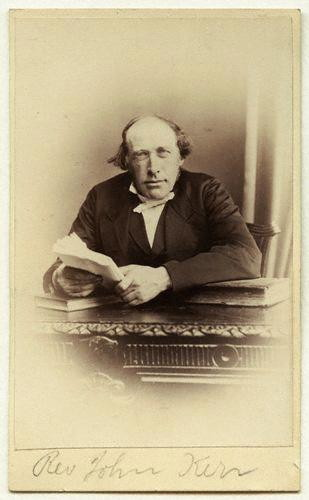
\includegraphics[scale = 0.35]{kerr}
		\caption{John Kerr, c. 1860, photograph by Thomas Annan}
	\end{figure}
	\par
	In the most basic terminology, refractive index of an optical medium defines the ability of that medium to change the path of light. Here, the definition of optical medium is crucial and so is the mathematical description of refractive index. For non-linear optical media, where the polarization density corresponds non-linearly to electric field of the light, the study of the propagation of light becomes quite involved. The principle of superposition, which follows from the Maxwell's equations, is no longer valid as the quantities like electric field are now dependent on parameters like dielectric constant. Non-linear optical media, thus, are remarkable as a plethora of new optical effects can be observed with such materials.
	\par
	On the other hand, a complex refractive index whose real part carries the refractive index and the imaginary part carries the absorption coefficient (also called as \textit{extinction}) can be defined. Now, if a high intensity beam of light is traversed through, the field due to this beam itself can produce changes in the refractive index and absorption coefficients of the material, and if we translate the material as the beam passes through it, we can record the changes as a function of distance. This forms the premise of the experiments that will follow from here, where we will translate materials along the path followed by a Nd-Yag laser beam being focused by a plano-convex lens. The direction in which the sample moves is the $ z $-direction, which gives the name for the technique. As the sample will move across the focus of the laser beam, a characteristic curve will be observed, which can be used to study the non-linear optical properties of the said material.
	



\section{Objectives}
	There are several major objectives that will be achieved as part of this experiment. They are:
	\begin{enumerate}
		\item To study the basics of non-
		linear optical properties by
		using Z-scan technique.
		\item Taking measurements of transmitted power for open and
		closed aperture by translating
		the material in the $ z $-direction.
		\item By fitting these data with the
		appropriate formulas, we will
		find the medium's nonlinear
		absorption coefficient and non-
		linear refractive index for different samples.
		\item To compare the difference between non-linear refractive index of a sample in two forms: as a \textit{thin film coating} and as a \textit{solution}. 
	\end{enumerate}


	
	

\section{Theory}
	When an electric field is applied across an electric insulator, polarization occurs within the insulator or the dielectric. This polarization density $ P $ is related to the applied electric field $ E $ as
	\begin{equation}
		\mathbf{P} = \varepsilon_0 \chi_e \mathbf{E}
	\end{equation}
	where $ \varepsilon_0 $ is the electric permittivity of free space and $ \chi_e $ is the electric susceptibility of the dielectric. Here, the relation between $ \mathbf{P} $ and $ \mathbf{E} $ is \textit{linear}, and thus the dielectrics which follow this relation are referred to as \textit{linear} (optical) mediums. More generally, for non-linear materials, we can write
	\begin{equation}\label{eq:2}
		\mathbf{P} = \varepsilon_0 \chi^{(1)} : \mathbf{E} + \varepsilon_0 \chi^{(2)} : \mathbf{EE} + \varepsilon_0 \chi^{(3)} : \mathbf{EEE} + \cdots
	\end{equation}
	Here $ \chi^{(n)} $ is the $ n $-th order component of the electric susceptibility of the medium which govern the non-linearities. The `:' symbol represents the scalar product between matrices. When the intensity of the light will be sufficiently high, only then
	these higher order polarization terms will be significant.
	

	\subsection{The Kerr effect}
		For a linear medium, only the first term of equation \eqref{eq:2} is significant and the polarization varies linearly with the electric field. For materials exhibiting a non-negligible Kerr effect, the third, $ \chi^{(3)} $ term is significant, with the even-order terms typically dropping out due to inversion symmetry of the Kerr medium (that is, in media with a center of symmetry).
		\par 
		If the beam of light is reasonably intense, which is true in case of lasers, the beam itself can provide the modulating electric field, without the need for an external field to be applied. Let the electric field $ \mathbf{E} $ in the case be
		\begin{equation}\label{key}
			\mathbf{E} = \mathbf{E}_{\omega} \cos (\omega t)
		\end{equation}
		with $ \mathbf{E_{\omega}} $ being the amplitude of the wave. Combining this with the equation for the polarization, and taking only linear terms and those in $ \chi^{(3)} |\mathbf{E_{\omega}}|^3$, we get
		\begin{equation}\label{key}
			\mathbf{P} = \varepsilon_0 \Big( \chi^{(1)} + \dfrac{3}{4}\chi^{(3)} |\mathbf{E_{\omega}}|^2 \Big) \mathbf{E_{\omega}} \cos (\omega t)
		\end{equation}
		This looks like a linear susceptibility with an additional non-linear term:
		\begin{equation}\label{key}
			\chi = \chi_{\mathrm{LIN}} + \chi_{\mathrm{NL}} = \chi^{(1)} + \dfrac{3}{4}\chi^{(3)} |\mathbf{E_{\omega}}|^2,
		\end{equation}
		and since the refractive index in terms of electric susceptibility is given by $ n = (1 + \chi)^{1/2}$, we have
		\begin{equation}\label{key}
			n = (1 + \chi_{\mathrm{LIN}} + \chi_{\mathrm{NL}})^{1/2} \simeq n_0 \Big( 1 + \dfrac{1}{2n_0^2} \chi_{\mathrm{NL}} \Big)
		\end{equation}
		where $ n_0 = (1 + \chi_{\mathrm{LIN}})^{1/2} $ is the linear refractive index. Using a Taylor expansion since $ \chi_{\mathrm{NL}} \ll n_0^2 $, this gives an \textit{intensity dependent refractive index} (IDRI) of:
		\begin{equation}\label{eq:7}
				n = n_0 + \dfrac{3 \chi^{(3)}}{8 n_0} |\mathbf{E_{\omega}}|^2
		\end{equation}
		As $ I = \frac{1}{2} \varepsilon_0 n_0 c |E_{\omega}|^2$, we obtain
		\begin{equation}\label{eq:8}
			\begin{split}
				n &= n_0 + \dfrac{3}{4} \chi^{(3)} \Big( \dfrac{I}{\varepsilon_0 n_0^2 c} \Big) \\
				\implies n &= n_0 + n_2 I
			\end{split}
		\end{equation}
		where $ n_2  = \frac{3 \chi^{(3)}}{4 \varepsilon_0 n_0^2 c}$  is the nonlinear component of the refractive index. This is known as the \textit{optical Kerr effect}.
	\subsection{The self-focusing and self-defocusing phenomena}
		The self focusing (or defocusing) of light beam is due to the
		dependence of the refractive index on the intensity of the beam. It is a non-linear optical processes induced by the
		change in refractive index of materials exposed to intense electromagnetic
		radiation. A medium whose refractive index increases with the electric field
		intensity acts as a focusing lens (Figure \ref{fig:focdefoc}a) for a Gaussian beam, while if it decreases with electric field intensity acts as defocusing lens (Figure \ref{fig:focdefoc}b).
		\begin{figure}
			\centering
			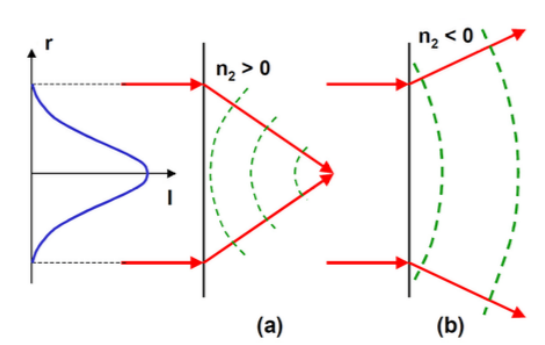
\includegraphics[scale = 0.7]{focdefoc}
			\caption{Self-focusing and defoucsing phenomena}
			\label{fig:focdefoc}
		\end{figure}


	\subsection{The Z-scan technique}
		Using a single Gaussian laser beam in a tight focus geometry, as depicted in Figure \ref{fig:schematic}, we measure the transmittance of a non-linear medium through a finite aperture in the fur field as a function of the sample position $ z $ measured with respect to the focal plane. Assume, for instance, a material with a negative nonlinear refractive index and a thickness smaller than the diffraction length of the focused beam (a thin medium). This can be regarded as a thin lens of variable focal length. Starting the scan from a distance far away from the focus (negative $ z $), the beam irradiance is low and negligible nonlinear refraction occurs; hence, the transmittance ($ D_2/D_1 $ in Figure \ref{fig:schematic}) remains relatively constant. As the sample is brought closer to focus, the beam irradiance increases, leading to self-focusing in the sample. A negative self-focusing prior to focus will tend to collimate the beam, causing a beam narrowing at the aperture which results in an increase in the measured transmittance. As the scan in $ z $ continues and the sample passes the focal plane to the right (positive $ z $), the same self-defocusing increases the beam divergence, leading to beam broadening at the aperture, and thus a decrease in transmittance. This suggests that there is a null as the sample crosses the focal plane. This is analogous to placing a thin lens at or near the focus, resulting in a minimal change of the far-field pattern of the beam. The Z-scan is completed as the sample is moved away from focus (positive $ z $) such that the transmittance becomes linear since the irradiance is again low.
		\begin{figure*}
			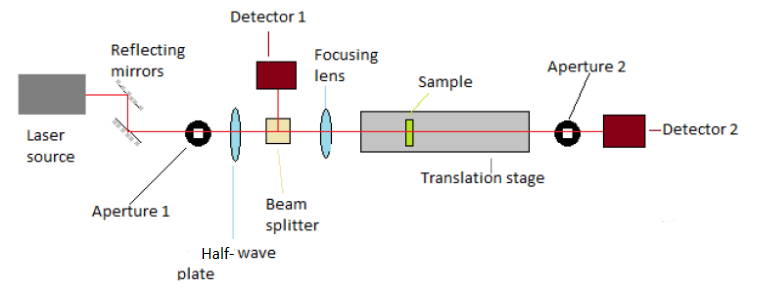
\includegraphics[scale = 1]{schematic}
			\caption{Schematic of the Z-scan setup}
			\label{fig:schematic}
		\end{figure*}
		\par 
		A prefocal transmittance maximum (peak) followed by a postfocal transmittance minimum (valley) is, therefore, the Z-scan signature of a negative refractive nonlinearity. Positive nonlinear refraction, following the same analogy, gives rise to an opposite valley-peak configuration.
		\par 
		When a high intensity laser beam propagates through a material, induced
		refractive index changes leads to self-focusing or defocusing of the laser beam
		which enables us to determine the third-order nonlinear optical properties of
		various materials. In this technique, the sample is translated along $ z $-direction through the beam waist of a focused beam by keeping the input power
		of beam constant. In our experiments a continuous pulse wave laser operating at 532 nm was used. The laser beam was focused using a $ \SI{10}{\centi \meter} $ focal length lens. Let us consider a material with positive non-linear refractive
		index, $ n_2 > 0 $. As shown in Fig. 1a), on the side of focus where the beam is
		converging, the non-linear lens shortens the beam's waist position to a negative $ z $ value. As the beam passes through the shifted focus, it diverges at
		a greater diffraction angle, so the beam's power is spread over a wider area
		and the intensity of beam passing through the pinhole decreases. When the
		sample is on the positive $ z $ side, where the beam is diverging, the non-linear
		lens reduces the beam's angle of divergence, thereby increasing the power
		passing through the pinhole. The effects are exactly opposite for $ n_2 < 0 $.
		\par 
		If the material has a positive non linearity ($ n_2 > 0 $), the transmittance
		graph has a valley first and then a peak. For the sample with $ n_2 < 0 $ the
		graph is exactly the opposite (first peak and then valley).
		\par 
		The aperture plays an important role in determining which values we are
		going to find. We use closed aperture for finding out the non-linear refractive
		index and open aperture to find the absorption coefficient.
		\begin{figure}
			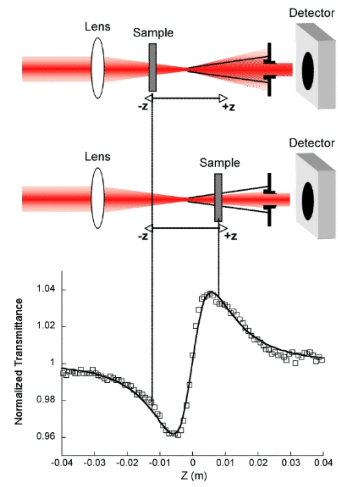
\includegraphics[scale = 0.7]{nlr}
			\caption{}
		\end{figure}
		\begin{figure}
			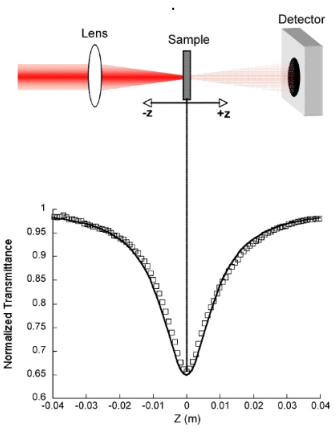
\includegraphics[scale = 0.7]{nla}
			\caption{}
		\end{figure}
		\begin{figure}
			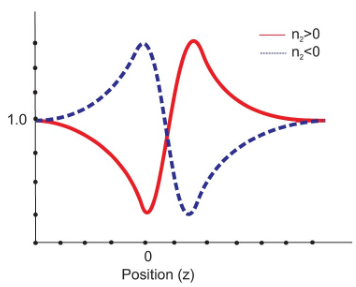
\includegraphics[scale = 0.8]{n2lg}
			\caption{}
		\end{figure}
	
	
	\subsection{Variation of optical properties with distance in non-linear media}\label{sec:der}
		Consider a $ \mathrm{TEM}_{00} $ Gaussian beam of beam waist radius $ w_0 $ travelling in the positive $ z $-direction, then the electric field $ E $ can be written as
		\begin{equation}\label{key}
			\begin{split}
				E (r, z, t) =& E_0 (t) \dfrac{w_0}{w(z)} \\
				& \cdot \exp \Bigg( -\dfrac{r^2}{w^2(z)} - \dfrac{ikr^2}{2 R(z)} \Bigg) e^{-i \phi (z, t)}
			\end{split}
		\end{equation}
		where $ w^2 (z) = w^2_0 (1 + z^2/z^2_0) $ is the beam radius, $ R(z) = z(1+z_0^2/z^2)$ is the radius of curvature of the wavefront at $ z $, $ z_0 = kw^2_0/2$ is the diffraction length of the beam, $ k = 2\pi/ \lambda $ is the wave vector, and $ \lambda $ is the laser wavelength, all in free space. $ E_0(t) $ denotes the radiation electric field at the focus and contains the temporal envelope of the laser pulse. The $ e^{-i \phi (z, t)} $ term contains all the radially uniform phase variations. As we are only concerned with calculating the radial phase variations $ \Delta \phi (r) $, the slowly varying envelope approximation (SVEA) applies, and all other phase changes that are uniform in $ r $ are ignored.
		\par 
		This beam is transmitted through a Kerr non-linear optical material of length $ L $, with a refractive index and absorption coefficient given by
		\begin{equation}\label{key}
			n(I) = n_0 + n_2 I.
		\end{equation}
		\begin{equation}\label{key}
			\alpha(I) = \alpha_0 + \beta I
		\end{equation}
		respectively, where: $ n_0 $ is the linear refractive index, $ n_2 $ is the non-linear refractive index, $ \alpha_0 $ is the absorption coefficient, $ \beta $ is the non-linear absorption coefficient and $ I $ is the intensity of light. The output field for a thin local media can then be written as
		\begin{equation}\label{eq:12}
			E_{out} = E(r, z)  e^{-\alpha_0 L/2} (1+q)^{(ikn_2/\beta - 1/2)}
		\end{equation}
		where $ q = \beta I L_{\mathrm{eff}} $ with $ L_{\mathrm{eff}} = (1-e^{-\alpha_0L})/\alpha_0 $. We also note that the on-axis intensity at beam waist is given by $ I_0 = |E_0|^2 $.For very thin samples, such as in this
		experiment, we can take $ L_{\mathrm{eff}} \approx 1 $ (in proper units). Moreover, $ I_{0} $ can be
		written as (see Appendix \ref{pulsed}):
		\begin{equation}\label{key}
			I_0 = \dfrac{\langle P \rangle}{f_{\mathrm{rep}} \tau \pi w_0^2}
		\end{equation}
		where $ \langle P \rangle $ is the average power of the beam, $ f_{\mathrm{rep}} $ is the repetition rate, $ \tau $ is the laser pulse width and $ \pi w_0^2 $ is the beam area at the focus.
		\par 
		Further, the irradiance distribution and phase shift of the beam at the exit surface of the sample must fulfill:
		\begin{equation}\label{key}
			I_{\mathrm{out}} (r,z) = \dfrac{I(r,z) e^{-\alpha_0L}}{1+q(r,z)}
		\end{equation}
		and
		\begin{equation}\label{eq:15}
			\Delta \phi = \dfrac{kn_2}{\beta} \ln (1+q(r,z))
		\end{equation}
		The intensity $ I $ can be expressed, at position $ z $, as the product of the maximum on axis value $ I_{0} $ and a Gaussian local profile ($ G_{\mathrm{loc}} $):
		\begin{equation}\label{key}
			I(r,z) = I_0 G_{\mathrm{loc}}
		\end{equation}
		with
		\begin{equation}\label{key}
			G_{\mathrm{loc}} = \dfrac{\exp(-2r^2/w^2(z))}{1+(z/z_0)^2}
		\end{equation}
		The field after a non-local sample that presents solely nonlinear refraction, the photoinduced non-linear phase change $ \Delta \phi_m $ can be written as:
		\begin{equation}\label{eq:18}
			\Delta \phi (r) = \Delta \Phi_0 G_{\mathrm{loc}}
		\end{equation}
		while for samples exhibiting solely non-linear absorption, $ q $ takes the following form:
		\begin{equation}\label{eq:19}
			q(r) = \Delta \Psi_0 G_{\mathrm{loc}}
		\end{equation}
		\par 
		From \eqref{eq:15}, it is evident that $ \Delta \Phi_0 $ and $ \Delta \Psi_0 $ are merely the results of the respective first order
		expansions of the expressions for $ \Delta \phi $  and $ q $, in the cases of pure
		non-linear refraction and pure non-linear absorption respectively. This gives us:
		\begin{equation}\label{key}
			 \Delta \Phi_0 = kn_2 I_0 L_{\mathrm{eff}}
		\end{equation}
		and
		\begin{equation}\label{key}
			\Delta \Psi_0 = 2^{-3/2} \beta I_0 L_{\mathrm{eff}}
		\end{equation}
		Substituting these quantities from \eqref{eq:18} and \eqref{eq:19} into \eqref{eq:12}, we
		obtain a final expression for the outgoing field:
		\begin{equation}\label{key}
			\begin{split}
				E_{\mathrm{out}} &= E(r,z) \exp (-\alpha_0 L/2) \\
				& \times [ 1+ \Delta \Psi_0 G_{\mathrm{loc}} ]^{-i(\Delta \Phi_0/\Delta \Psi_0)-1/2}
			\end{split}
		\end{equation}
		\par 
		Now, making use of SVEA and the Gaussian decomposition method for
		local field changes and considering only the first two terms in the decomposition, we can obtain an analytical expression for the complex, on-axis far-field as:
		\begin{equation}\label{eq:23}
			\begin{split}
				E_{\mathrm{out}} &= E(r,z) \exp (-\alpha_0 L/2) \\
				& \times \sum_{n=0}^{\infty} \Bigg[ \dfrac{(-i \Delta \phi_0(z))^n}{n!} \times \prod_{n'=0}^{n}\Bigg( 1 - i(2n'-1)\dfrac{\Delta \Psi_0}{\Delta \Phi_0} \Bigg) \Bigg] \\
				& \times \exp \Bigg( \dfrac{-2nr^2}{w^2(z)} \Bigg)
			\end{split}
		\end{equation}
		Using \eqref{eq:23} we can write the complex field at the aperture planes as
		follows:
		\begin{equation}\label{eq:24}
			\begin{split}
				E_{a} &= E(r,z) \sum_{n=0}^{\infty} \dfrac{(-i \Delta \phi_0(z))^n}{n!} \\
				& \times \prod_{n'=0}^{n}\Bigg( 1 - i(2n'-1)\dfrac{\Delta \Psi_0}{\Delta \Phi_0} \Bigg) \dfrac{w_{n0}}{w_n} \\
				& \times \exp \Bigg( \dfrac{-r^2}{w_n^2} - \dfrac{ikr^2}{2R_n} + i \theta_n \Bigg)
			\end{split}
		\end{equation}
		Here $ \Delta \phi_0 = \Delta \Phi_0 /(1+(z/z_0)^2) $. When only non-linear refraction is considered, $ \Delta \Psi_0 \rightarrow 0 $, and we can reduce \eqref{eq:24} to obtain:
		\begin{equation}\label{eq:25}
			\begin{split}
				E_{a} &= E(r,z) \sum_{n=0}^{\infty} \dfrac{(-i \Delta \phi_0(z))^n}{n!} \\
				& \times \dfrac{w_{n0}}{w_n} \exp \Bigg( \dfrac{-r^2}{w_n^2} - \dfrac{ikr^2}{2R_n} + i \theta_n \Bigg)
			\end{split}
		\end{equation}
		\par 
		Taking $ d $ to be the propagation distance in free space, between the sample
		and the aperture, and $ g = 1 + d/R(z) $, we can represent the parameters in
		\eqref{eq:24} and \eqref{eq:25} as follows:
		\begin{center}
			$ w_{n0}^2 = \dfrac{w^2(z)}{2n+1}$, \\

			$ d_n = \dfrac{kw_{n0}^2}{2} $, \\

			$ w_n^2 = w^2_{n0} \Bigg( g^2 \dfrac{d^2}{d_n^2} \Bigg)$, \\

			$ R_n^2 = d \Bigg(1-\dfrac{g}{g^2 + (d/d_n)^2}\Bigg)^{-1} $
		\end{center}
		and,
		\begin{center}
			$ \theta_n = \tan^{-1} \Big(\dfrac{d}{gd_n}\Big) $
		\end{center}
		\par 
		The total transmitted power through the aperture can then be obtained
		by spatially integrating $ E_a(r, t) $:
		\begin{equation}\label{key}
			P_T (\Delta \Phi_0 (t)) = \int_{0}^{r_a} |E_a(r,t)|^2 r dr
		\end{equation}
		This directly yields the normalized Z-scan transmittance, $ T(z) $, using the
		following expression:
		\begin{equation}\label{key}
			T(z) = \dfrac{\int_{-\infty}^{\infty} P_T (\Delta \Phi_0 (t)) dt}{S \int_{-\infty}^{\infty} P_i (t) dt}
		\end{equation}
		where $ P_i(t) = \pi w_0^2 I_0 (t)/2 $ is the instantaneous input power, within the sample, and $ S = 1 - \exp(-2r_a^2/w_a^2) $, where subscript $ a $ denotes `aperture'.
		This is where the aperture-dependence of the Z-Scan traces comes in. For
		closed aperture traces, we can take $ S \approx 0 $ and for open aperture traces,
		$ S \approx 1 $. Now, the normalized transmittance for the on-axis electric field, at
		the aperture plane, can be written as:
		\begin{equation}\label{eq:28}
			T_2 (z, \Delta \phi_0) = \dfrac{\Big|E(r=0,z,\Delta \phi_0)\Big|^2}{\Big|E(r=0,z,\Delta \phi_0=0)\Big|^2}
		\end{equation}
		On substituting the expression for the field into \eqref{eq:28} and simplifying, we
		obtain the final expression for $ T(z) $,
		that considers the effect of both non-linear refraction and non-linear absorption, as given below:
		\begin{equation}\label{eq:29}
			T_2(z, \Delta \Phi_0, \Delta \Psi_0) = 1 + \dfrac{4 \Delta \Phi_0 z}{(z^2+9)(z^2+1)} - \dfrac{\Delta \Psi_0}{z^2+1}
		\end{equation}
		\par 
		Equation \eqref{eq:29} provides a two-parameter fitting function for any third-order Z-
		scan trace, the two parameters being $ \Delta \Phi_0 $ and $ \Delta \Psi_0 $, and we have used it
		to fit the closed aperture traces, in order to obtain the $ n_2 $ values in this
		experiment. On the other hand, for $ \beta $ values, we take the open aperture
		traces, that deemphasize $ \Delta \Phi_0 $ or small intensity variations, as the entire
		signal is being measured.
		So, we can provide a simpler, one-parameter
		expression for $ T(z) $ in this case:
		\begin{equation}\label{eq:30}
			T_2(z, \Delta \Phi_0=0, \Delta \Psi_0) = 1 - \dfrac{\Delta \Psi_0}{z^2+1}
		\end{equation}
		\par 
		Equations \eqref{eq:29} and \eqref{eq:30} are the working formulae for this experiment. Figure 4
		shows variations in transmittance in Z-scan traces for materials exhibiting
		pure non-linear refraction, pure non-linear absorption and both (mixed case), using various
		values for $ \Delta \Phi_0 $ and $ \Delta \Psi_0 $. It is clear from the plots that non-linear absorption suppresses
		peaks in the mixed Z-Scan traces, as compared to the pure non-linear refraction case. This
		also means that the symmetric nature of pure non-linear refraction curves is usually absent
		in most Z-Scan traces, where both non-linear refraction and non-linear absorption contribute. As such, we
		can utilize another interesting quantity, that is the Peak-Valley Transmittance Change, $ \Delta T_{p-v} $. It is expressed as follows in the closed aperture case
		(where we shall be using the two-parameter fitting function in \eqref{eq:29}):
		\begin{equation}\label{key}
			\Delta T_{p-v} = 0.406 \Delta \Phi_0
		\end{equation}
		This relation for $ \Delta T_{p-v} $ should hold even for highly skewed Z-Scan traces.
		Therefore, it provides us with an excellent tool to verify the quality of our
		traces.
		
		
		
		
\section{The Experiments}
	In this section, we will describe the experimental set-up, how various apparatus are arranged after alignment of the laser, explain the basic scientific principle of the technique and methodology of how they were performed.
	\subsection{Experimental set-up}
	The various apparatus and their working in Figure \ref{fig:schematic} is explained in this section.
	\begin{enumerate}
		\item \textbf{Laser Source}: We
		use
		the
		pulsed $ \SI{532}{\nano \meter} $ laser.
		\item We used the two reflecting mirrors for aligning the beam by
		parallel
		(Z-fold) (Figure \ref{fig:zfold})
		configuration.
		\begin{figure}
			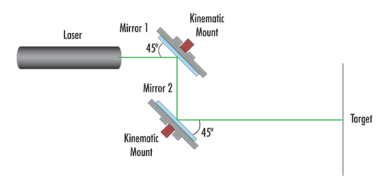
\includegraphics{zfold}
			\caption{Z-fold configuration of  reflecting mirrors}
			\label{fig:zfold}
		\end{figure}
		\item \textbf{Wave plate}:
		Optical device
		which alter the polarization
		state of light wave traveling
		through it. There are two types
		of wave plate, first half wave
		plate which shift the polarization direction of linearly polarized light, second is quarter
		wave plate which converts linearly polarized light into circularly polarized light. Here, we have used a half-wave plate.
		\item \textbf{Beam Splitter}:
		Optical components used to split incident light at a designated ratio into
		two separate beams.
		There
		will be semi reflective coating
		on one of the prism.
		Ratio of reflection/transmission
		depends on coating material.
		There are two type of beam-splitter, first is polarizing beam
		splitter(divides incident unpolarized light into orthogonal
		polarized beams) and second
		is non-polarized beam splitter (split by specific percentage
		that is independent of polarization).
		\item\textbf{ Thermal detectors}: It is based
		on temperature change of the element through the absorption of EM radiation. Change
		in temperature causes change
		in
		temperature
		dependent
		property (resistance) of thermal detector, which is evaluated electrically and is measure
		of the absorbed energy.
		\item A converging Lens ($ L_0 $), with
		$ f = \SI{10}{\centi \metre} $, to focus the LASER
		light.
		\item A translation stage
		\item A beam profiler to measure the
		beam waist.
		\item An optical table to assemble
		the setup.
		\item Allen keys and bolts to hold
		the equipment in place.
		\item Multiple screens to avoid interference from other setups.
	\end{enumerate}
	We are using a combination of wave plate and beam-
	splitter to control the intensity of laser beam.
	Through
	half-waveplate we will bring a
	polarisation in the light and
	our beam splitter will split
	the beam intensity (will reflect
	some and pass some) as per polarisation.
	\subsection{Observations}
	The specifications of the laser and some other quantities that were kept fixed are given below:
	\begin{enumerate}
		\item Effective length of the sample, $ L_{\mathrm{eff}} = \SI{1}{\milli \meter} $,
		\item Repetition rate of the laser, $ f_{\mathrm{rep}} = \SI{6}{\kilo \hertz}$,
		\item Pulse width at a given repetition rate, $ \tau = \SI{500}{\pico \second} $,
		\item Beam waist width of the laser beam, $ w_0 = \SI{20}{\micro \meter} $
	\end{enumerate}
	\par 
	In the following sections, the variation of transmittance with distance from the focus is plotted from the electronically recorded data. Using the relevant equations derived in Section \ref{sec:der}, we have calculated the second order non-linear refractive index or the non-linear absorption coefficient (whichever is applicable). The error analysis is performed using Python libraries. The code for the same is publicly available at my \href{https://github.com/peakcipher/coursework/tree/master/22O1}{GitHub}.
	
	
	\subsection{With Toluene solution}
		\subsubsection{Closed Aperture}
			After fitting the recorded data according to \eqref{eq:29} the following observations were made:
			\begin{enumerate} 
				\item Average power, $ \langle P \rangle  = \SI{60}{\milli \watt}$
				\item Second order non-linear refractive index, $ n_2 = \SI[separate-uncertainty=true]{-3.3 \pm 0.7e-18}{\meter \squared \per \watt} $.
			\end{enumerate}
			\begin{figure}
				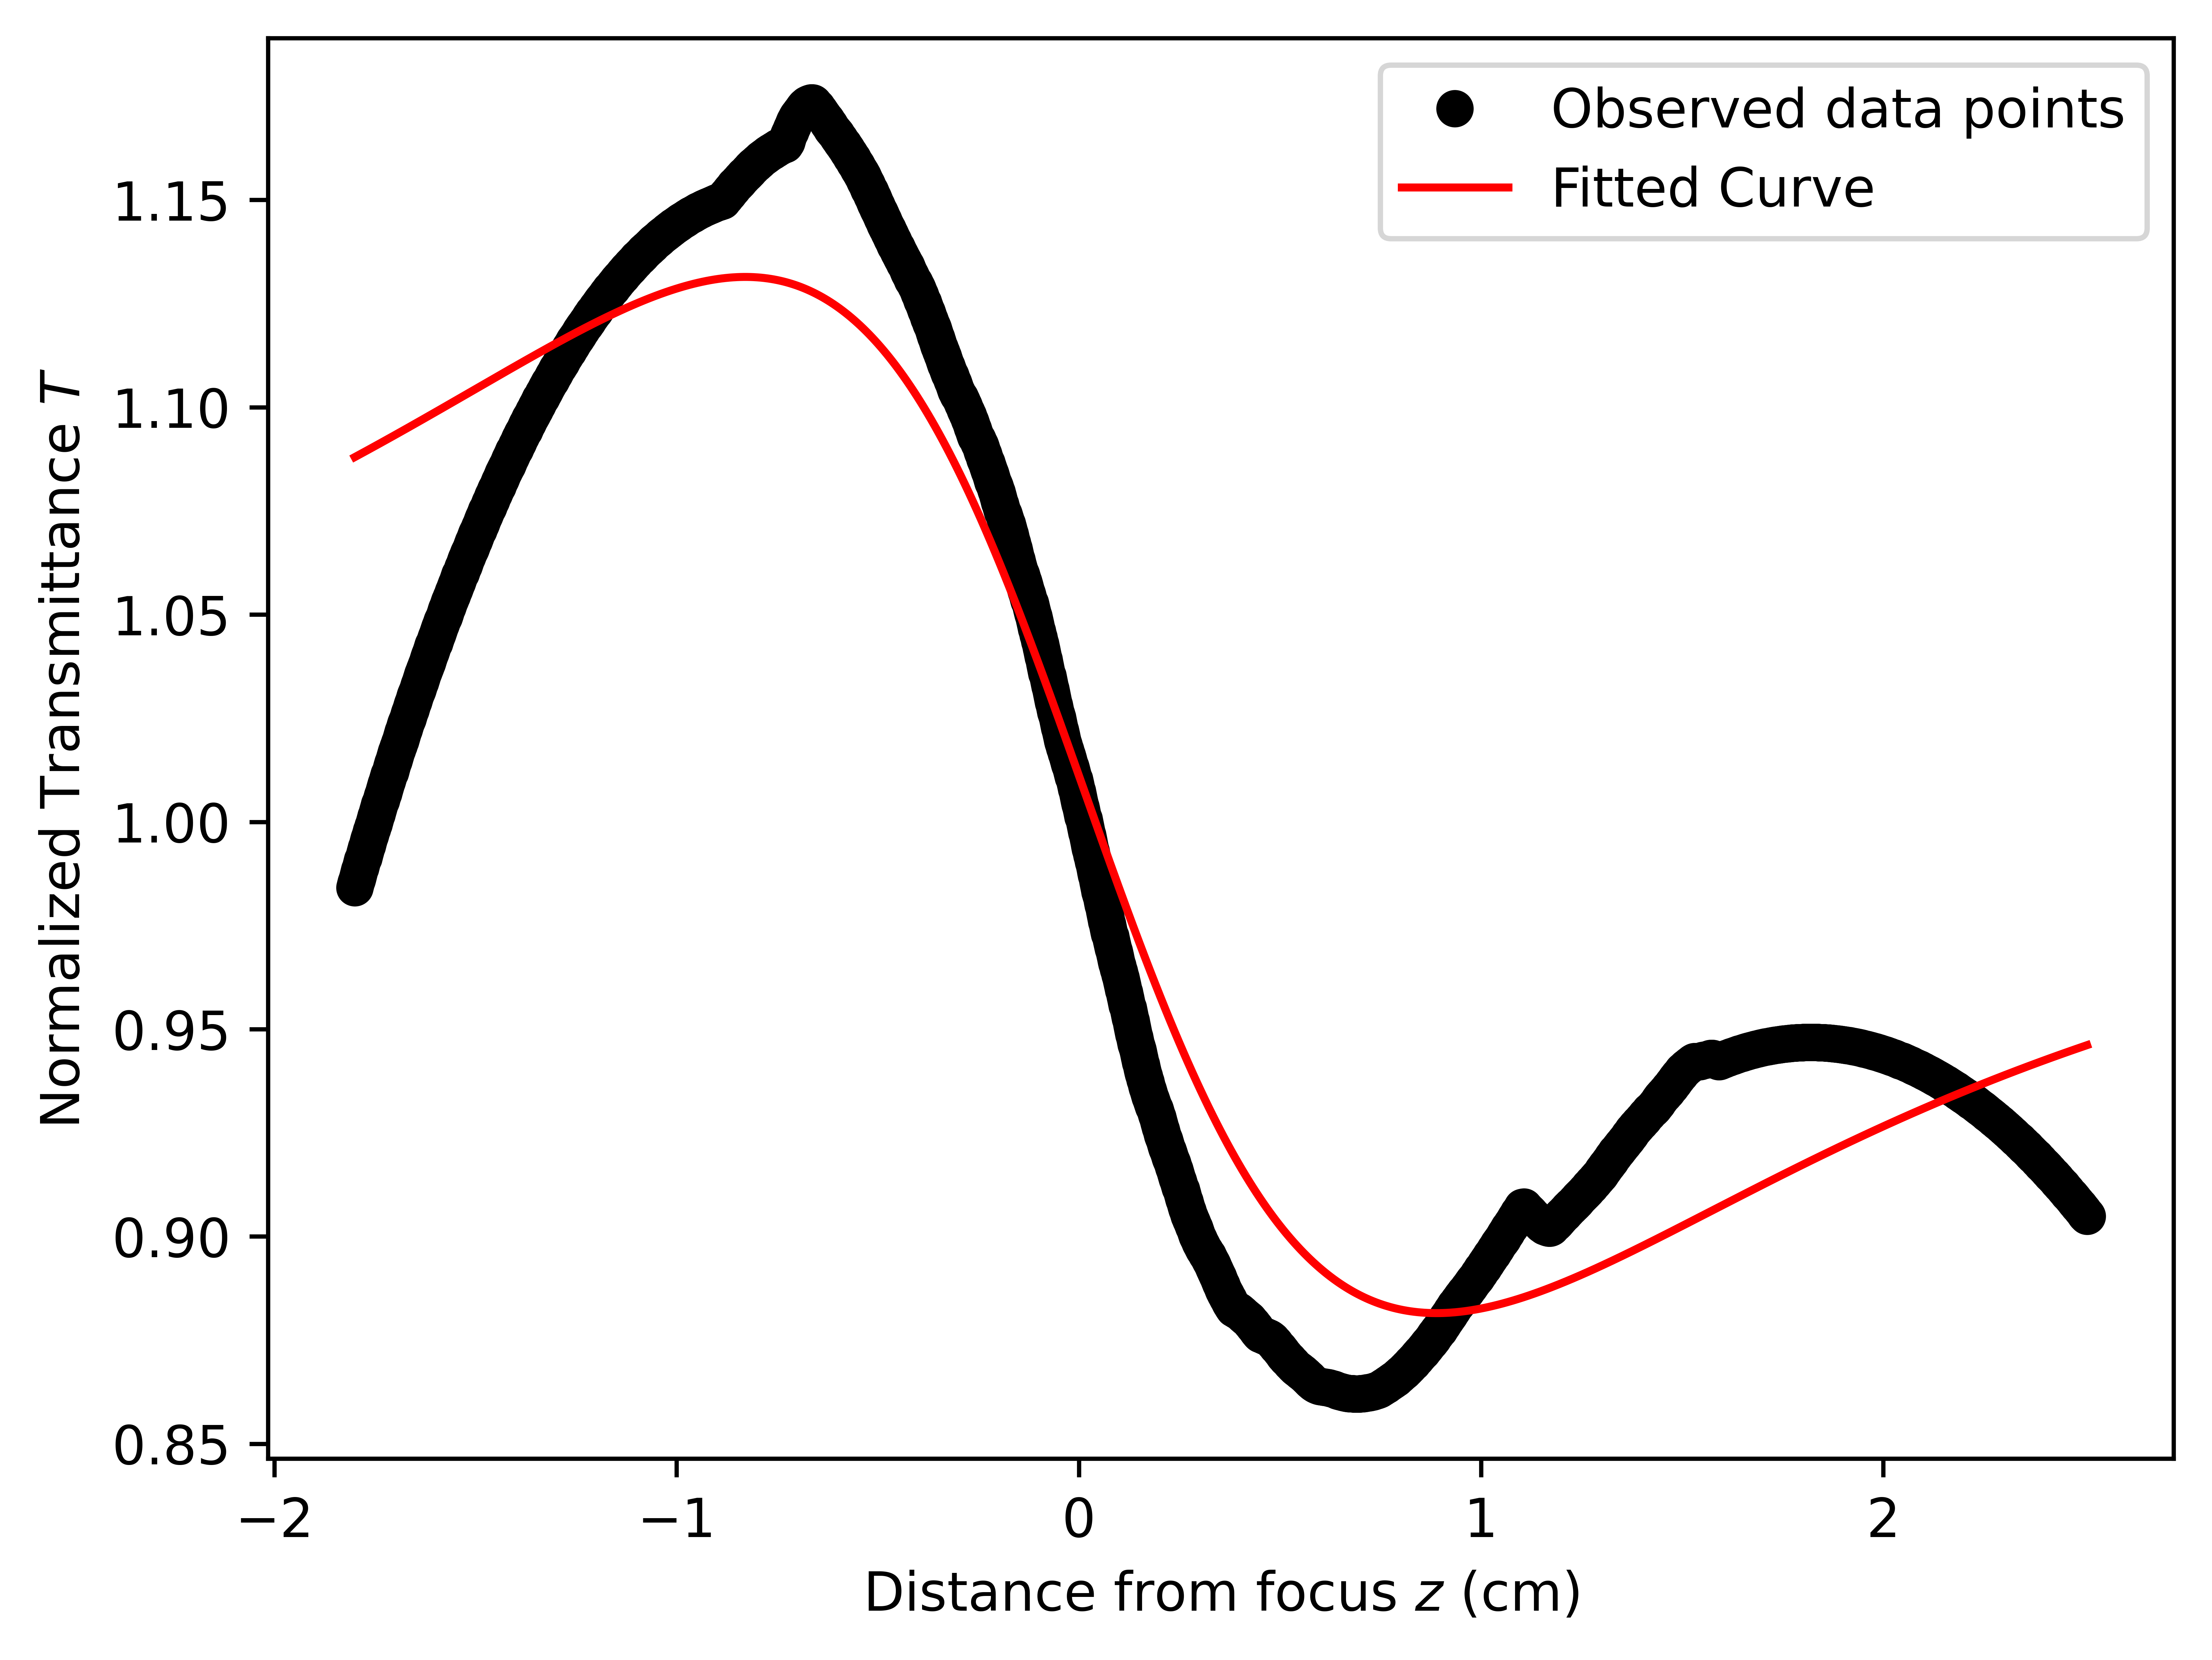
\includegraphics[scale = 0.59]{tol-c}
				\caption{Variation of transmittance with distance for toluene solution (closed aperture)}
			\end{figure}
		
		\subsubsection{Open Aperture}
		After fitting the recorded data according to \eqref{eq:30} the following observations were made:
		\begin{enumerate} 
			\item Average power, $ \langle P \rangle  = \SI{60}{\milli \watt}$
			\item Non-linear absorption coefficient, $ \beta = \SI[separate-uncertainty=true]{6.0 \pm 1.3e-18}{\meter \per \watt} $.
		\end{enumerate}
		\begin{figure}
			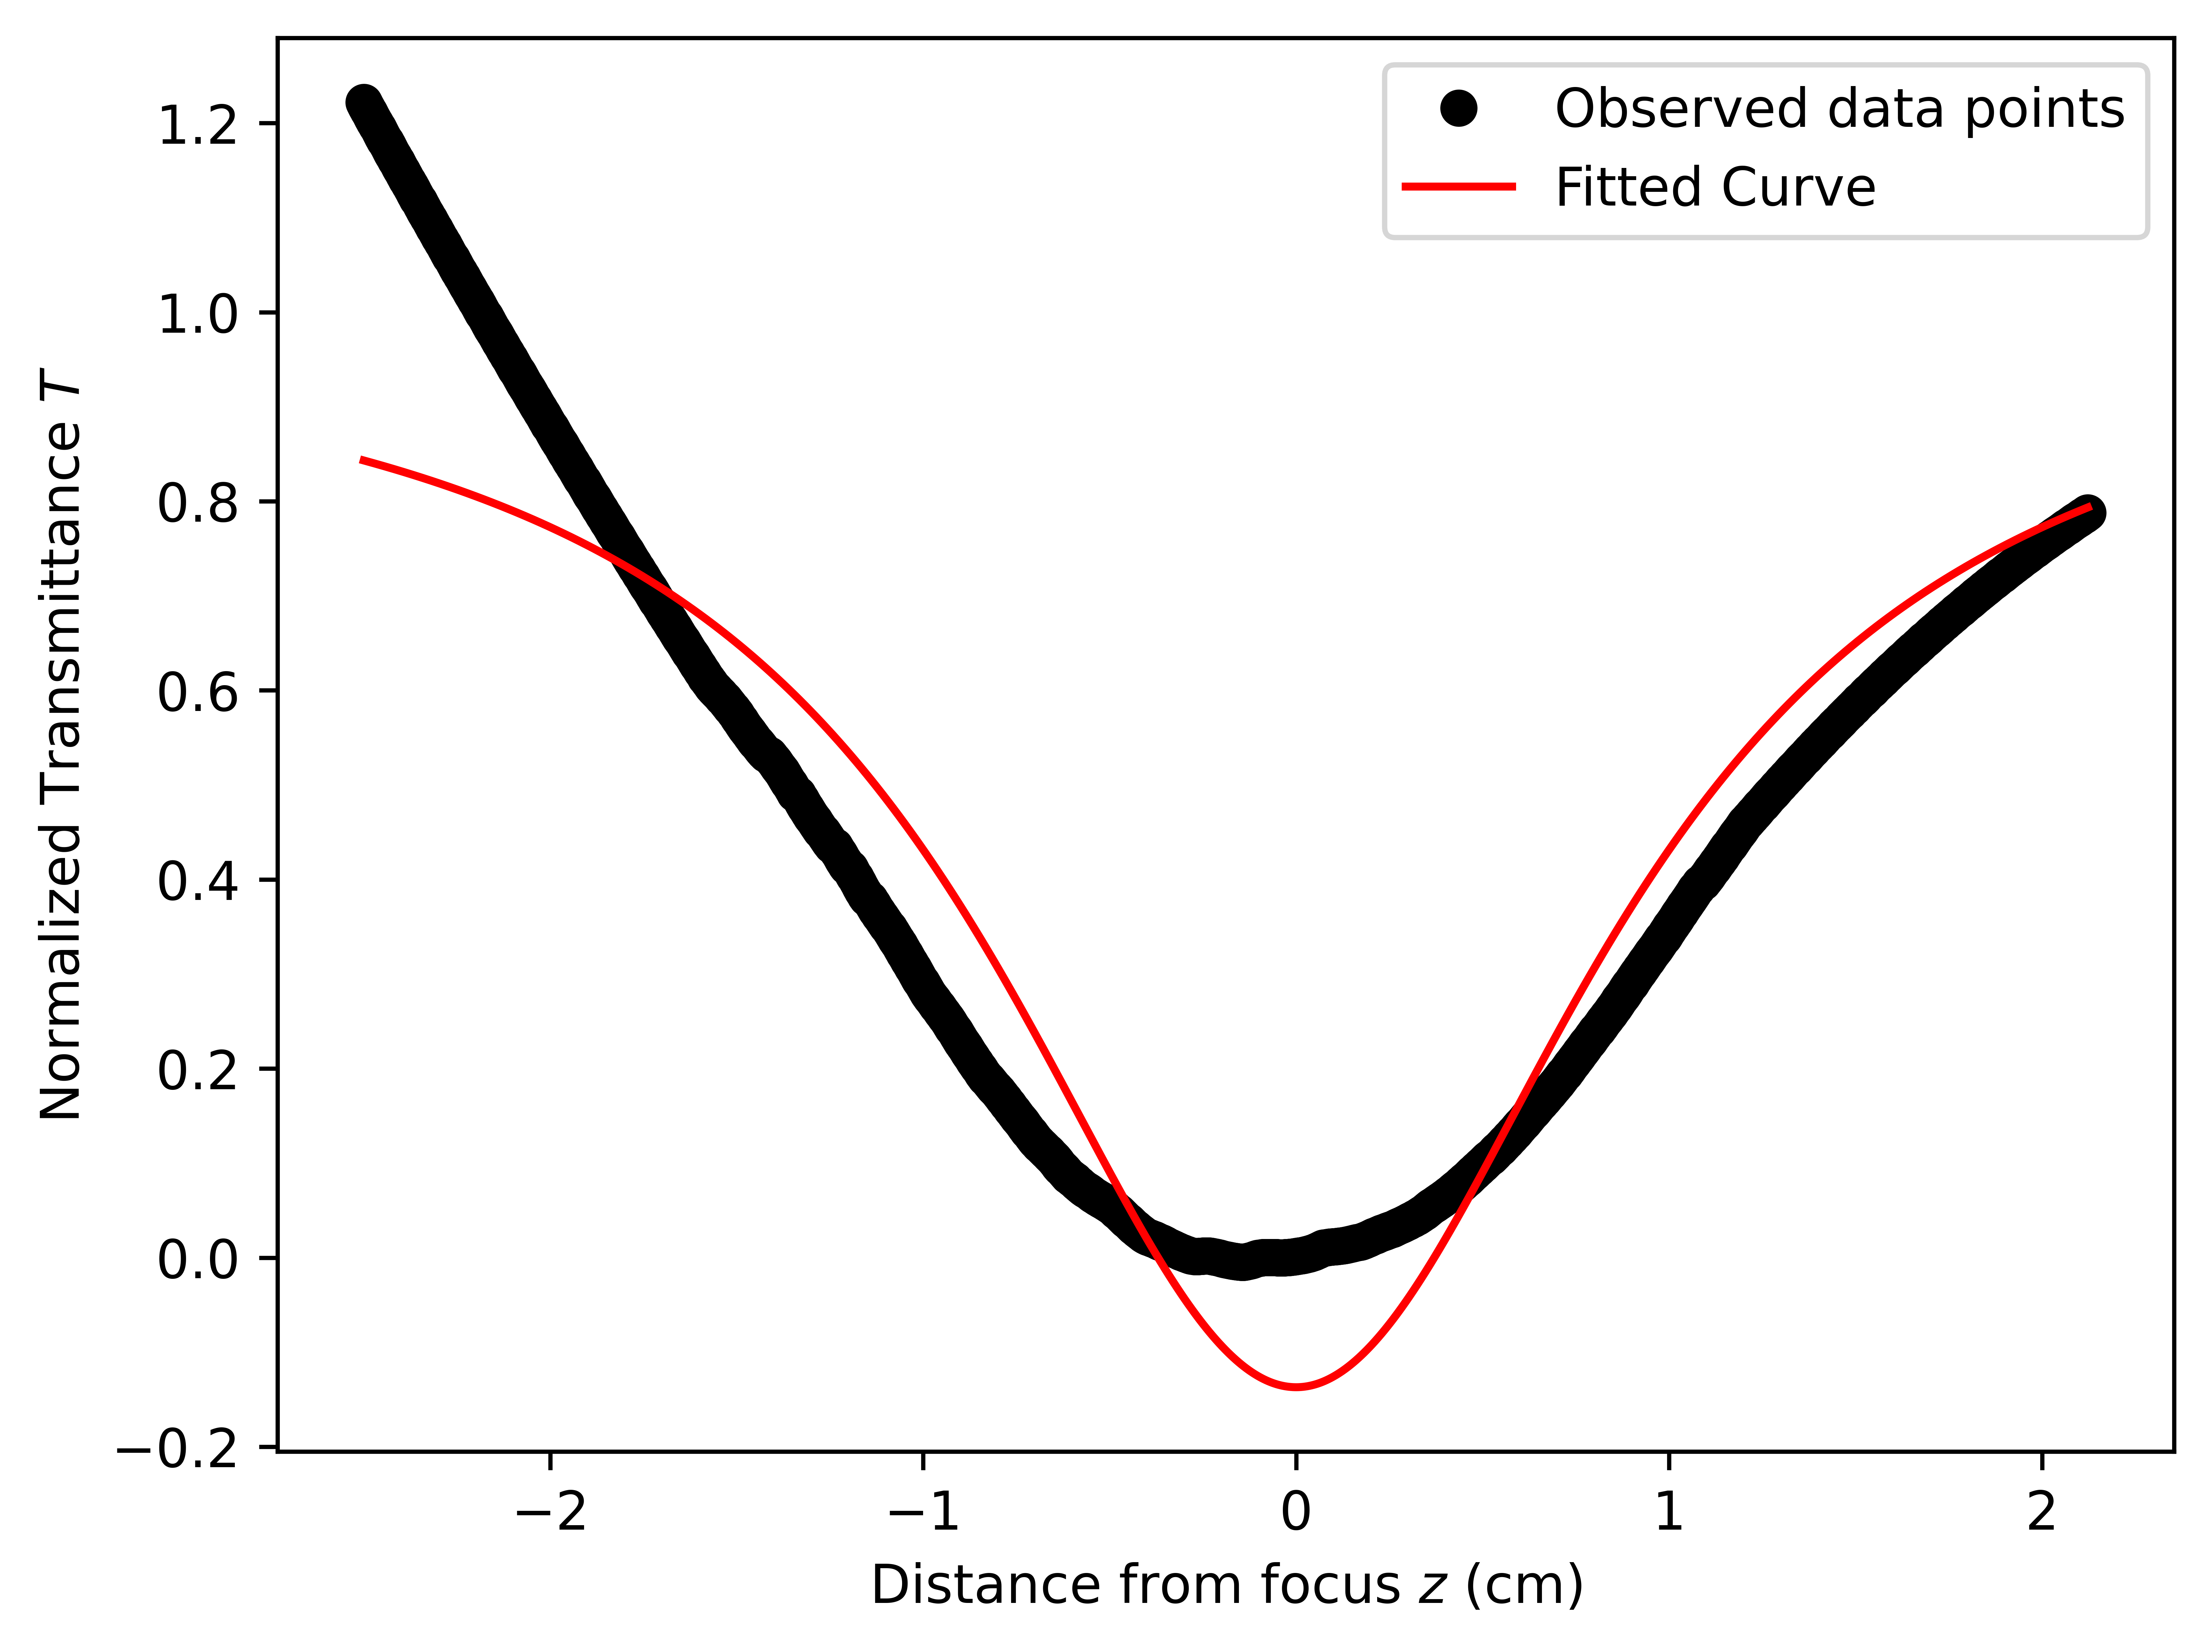
\includegraphics[scale = 0.59]{tol-o}
			\caption{Variation of transmittance with distance for toluene solution (open aperture)}
		\end{figure}
		
		
		
		
		
		
	\subsection{With methyl ammonium lead iodide thin film}
		\subsubsection{Closed Aperture}
		After fitting the recorded data according to \eqref{eq:29} the following observations were made:
		\begin{enumerate} 
			\item Average power, $ \langle P \rangle  = \SI{180}{\milli \watt}$
			\item Second order non-linear refractive index, $ n_2 = \SI[separate-uncertainty=true]{-1.05 \pm 0.23e-18}{\meter \squared \per \watt} $.
		\end{enumerate}
		\begin{figure}
			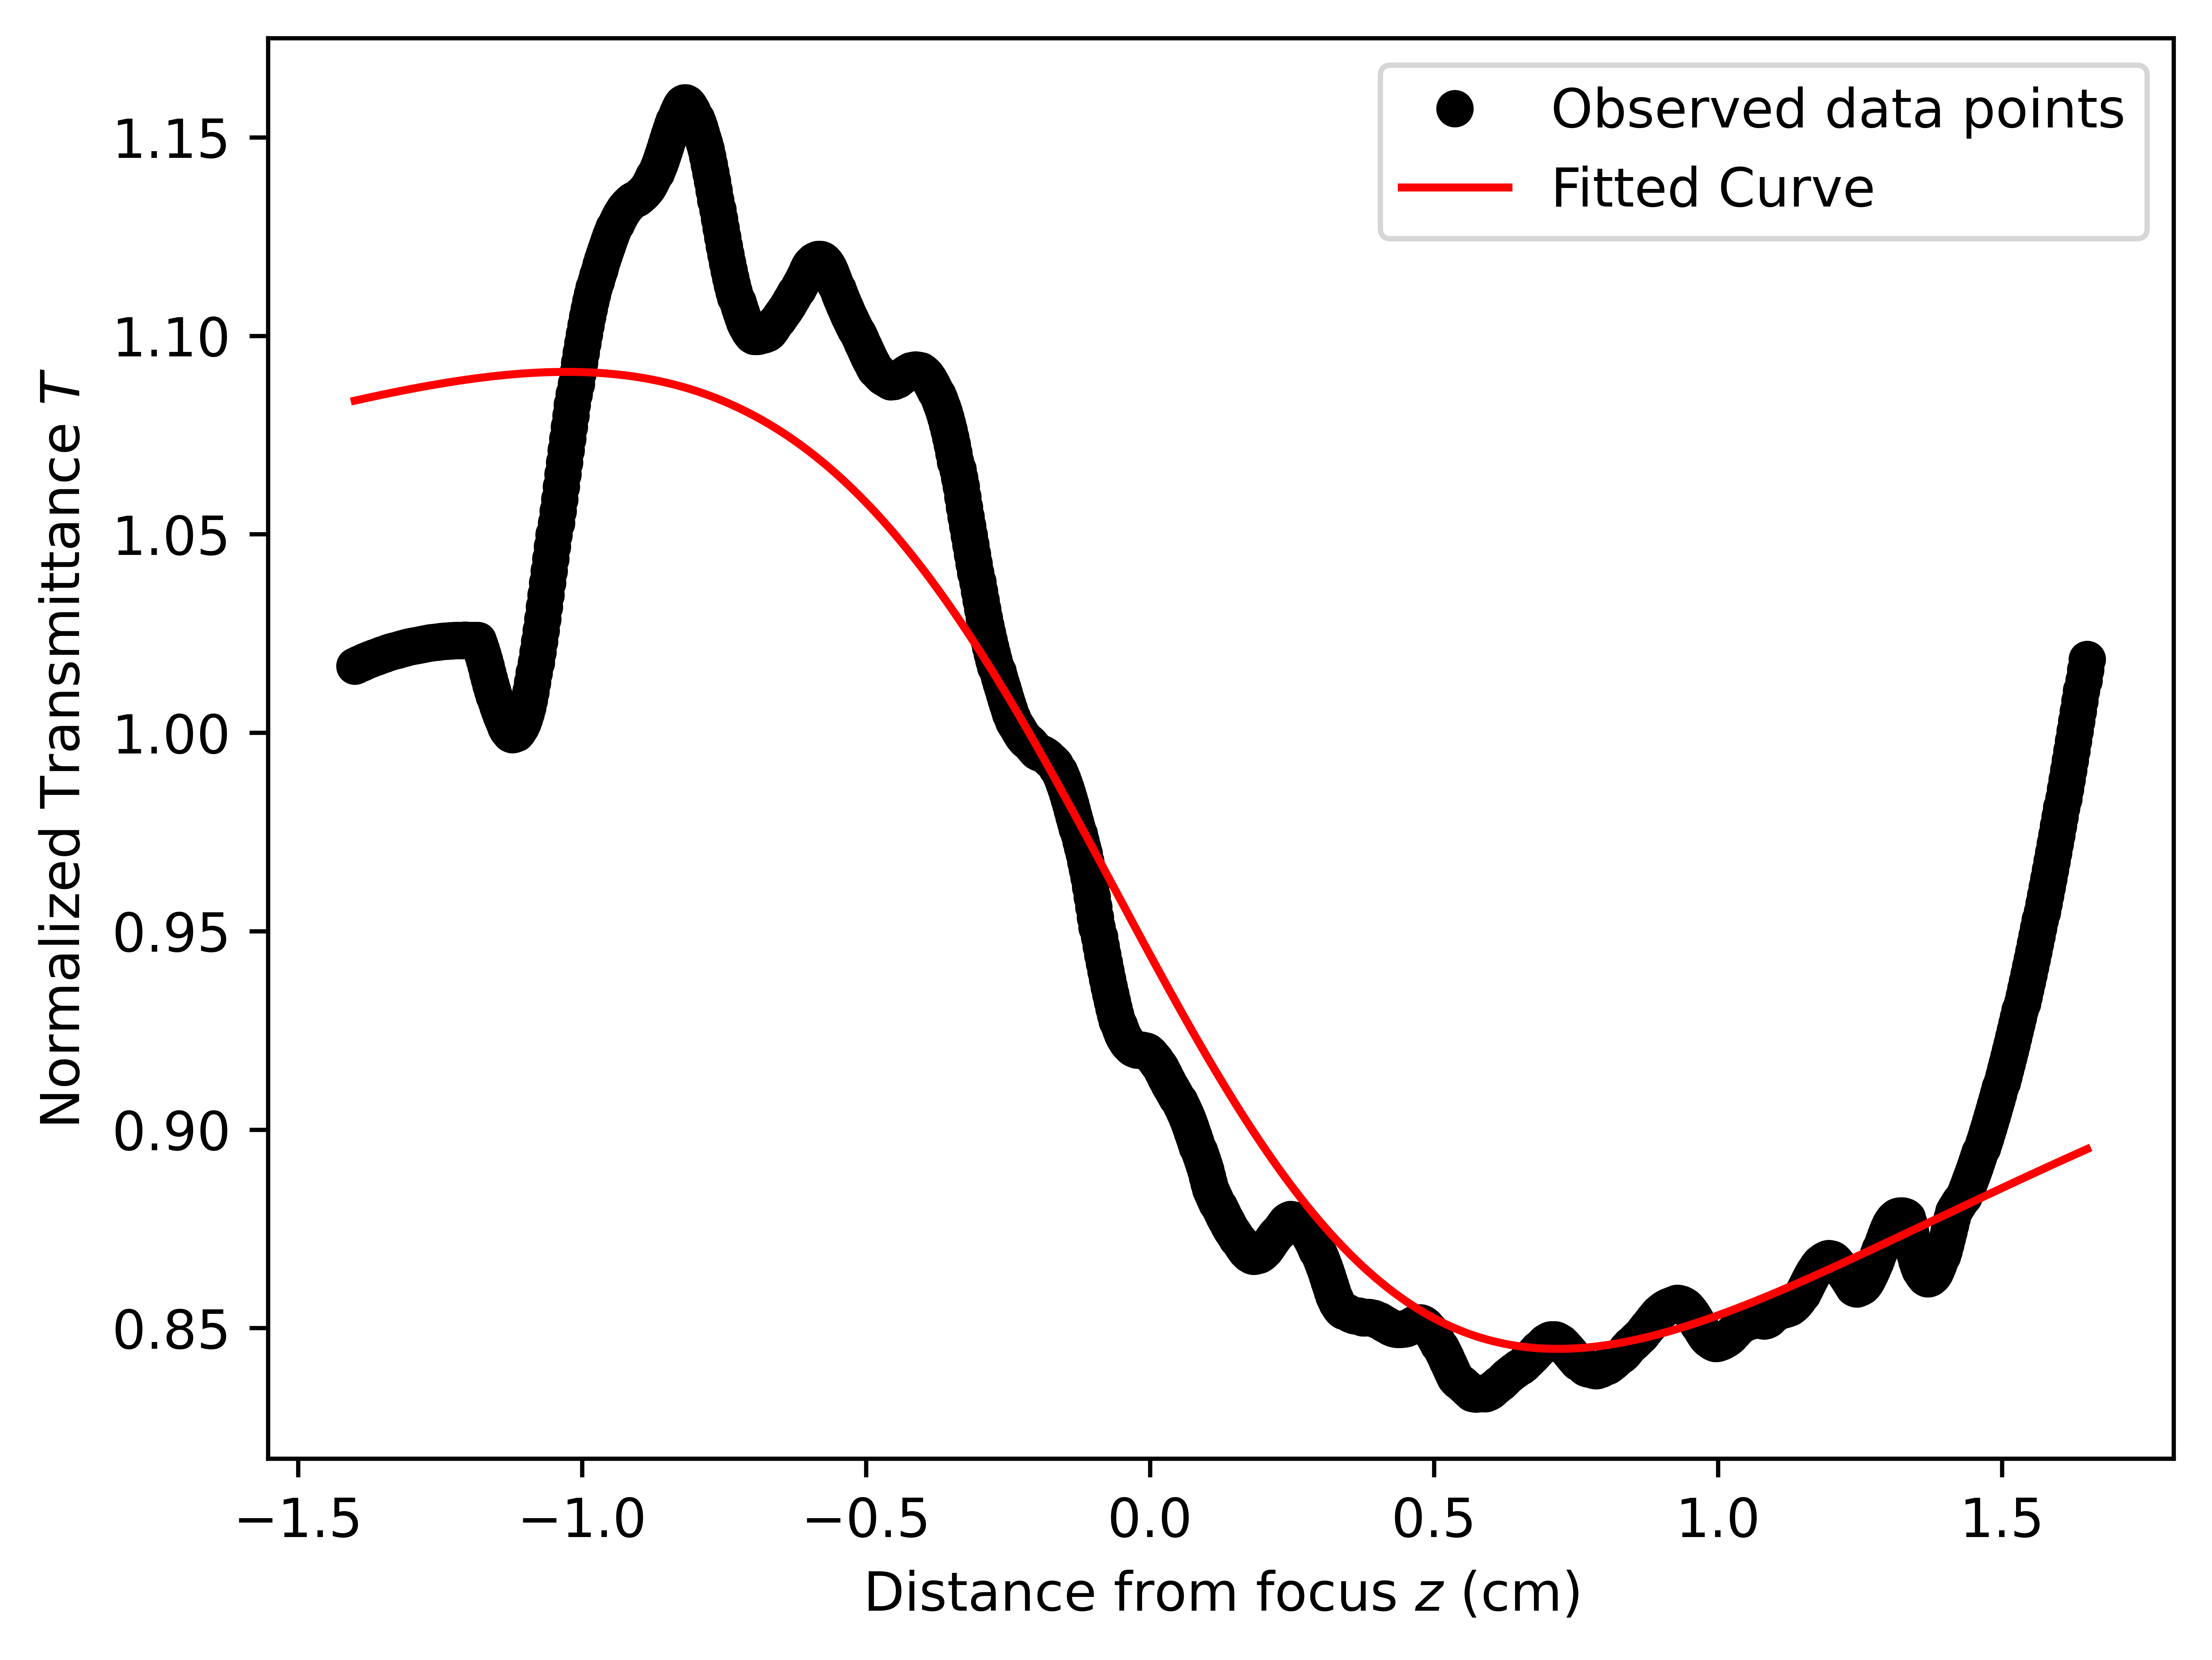
\includegraphics[scale = 0.59]{satys-c}
			\caption{Variation of transmittance with distance for methyl ammonium lead iodide thin film (closed aperture)}
		\end{figure}
		
		\subsubsection{Open Aperture}
		After fitting the recorded data according to \eqref{eq:30} the following observations were made:
		\begin{enumerate} 
			\item Average power, $ \langle P \rangle  = \SI{80}{\milli \watt}$
			\item Non-linear absorption coefficient, $ \beta = \SI[separate-uncertainty=true]{-3.4 \pm 0.7e-18}{\meter \per \watt} $.
		\end{enumerate}
		\begin{figure}
			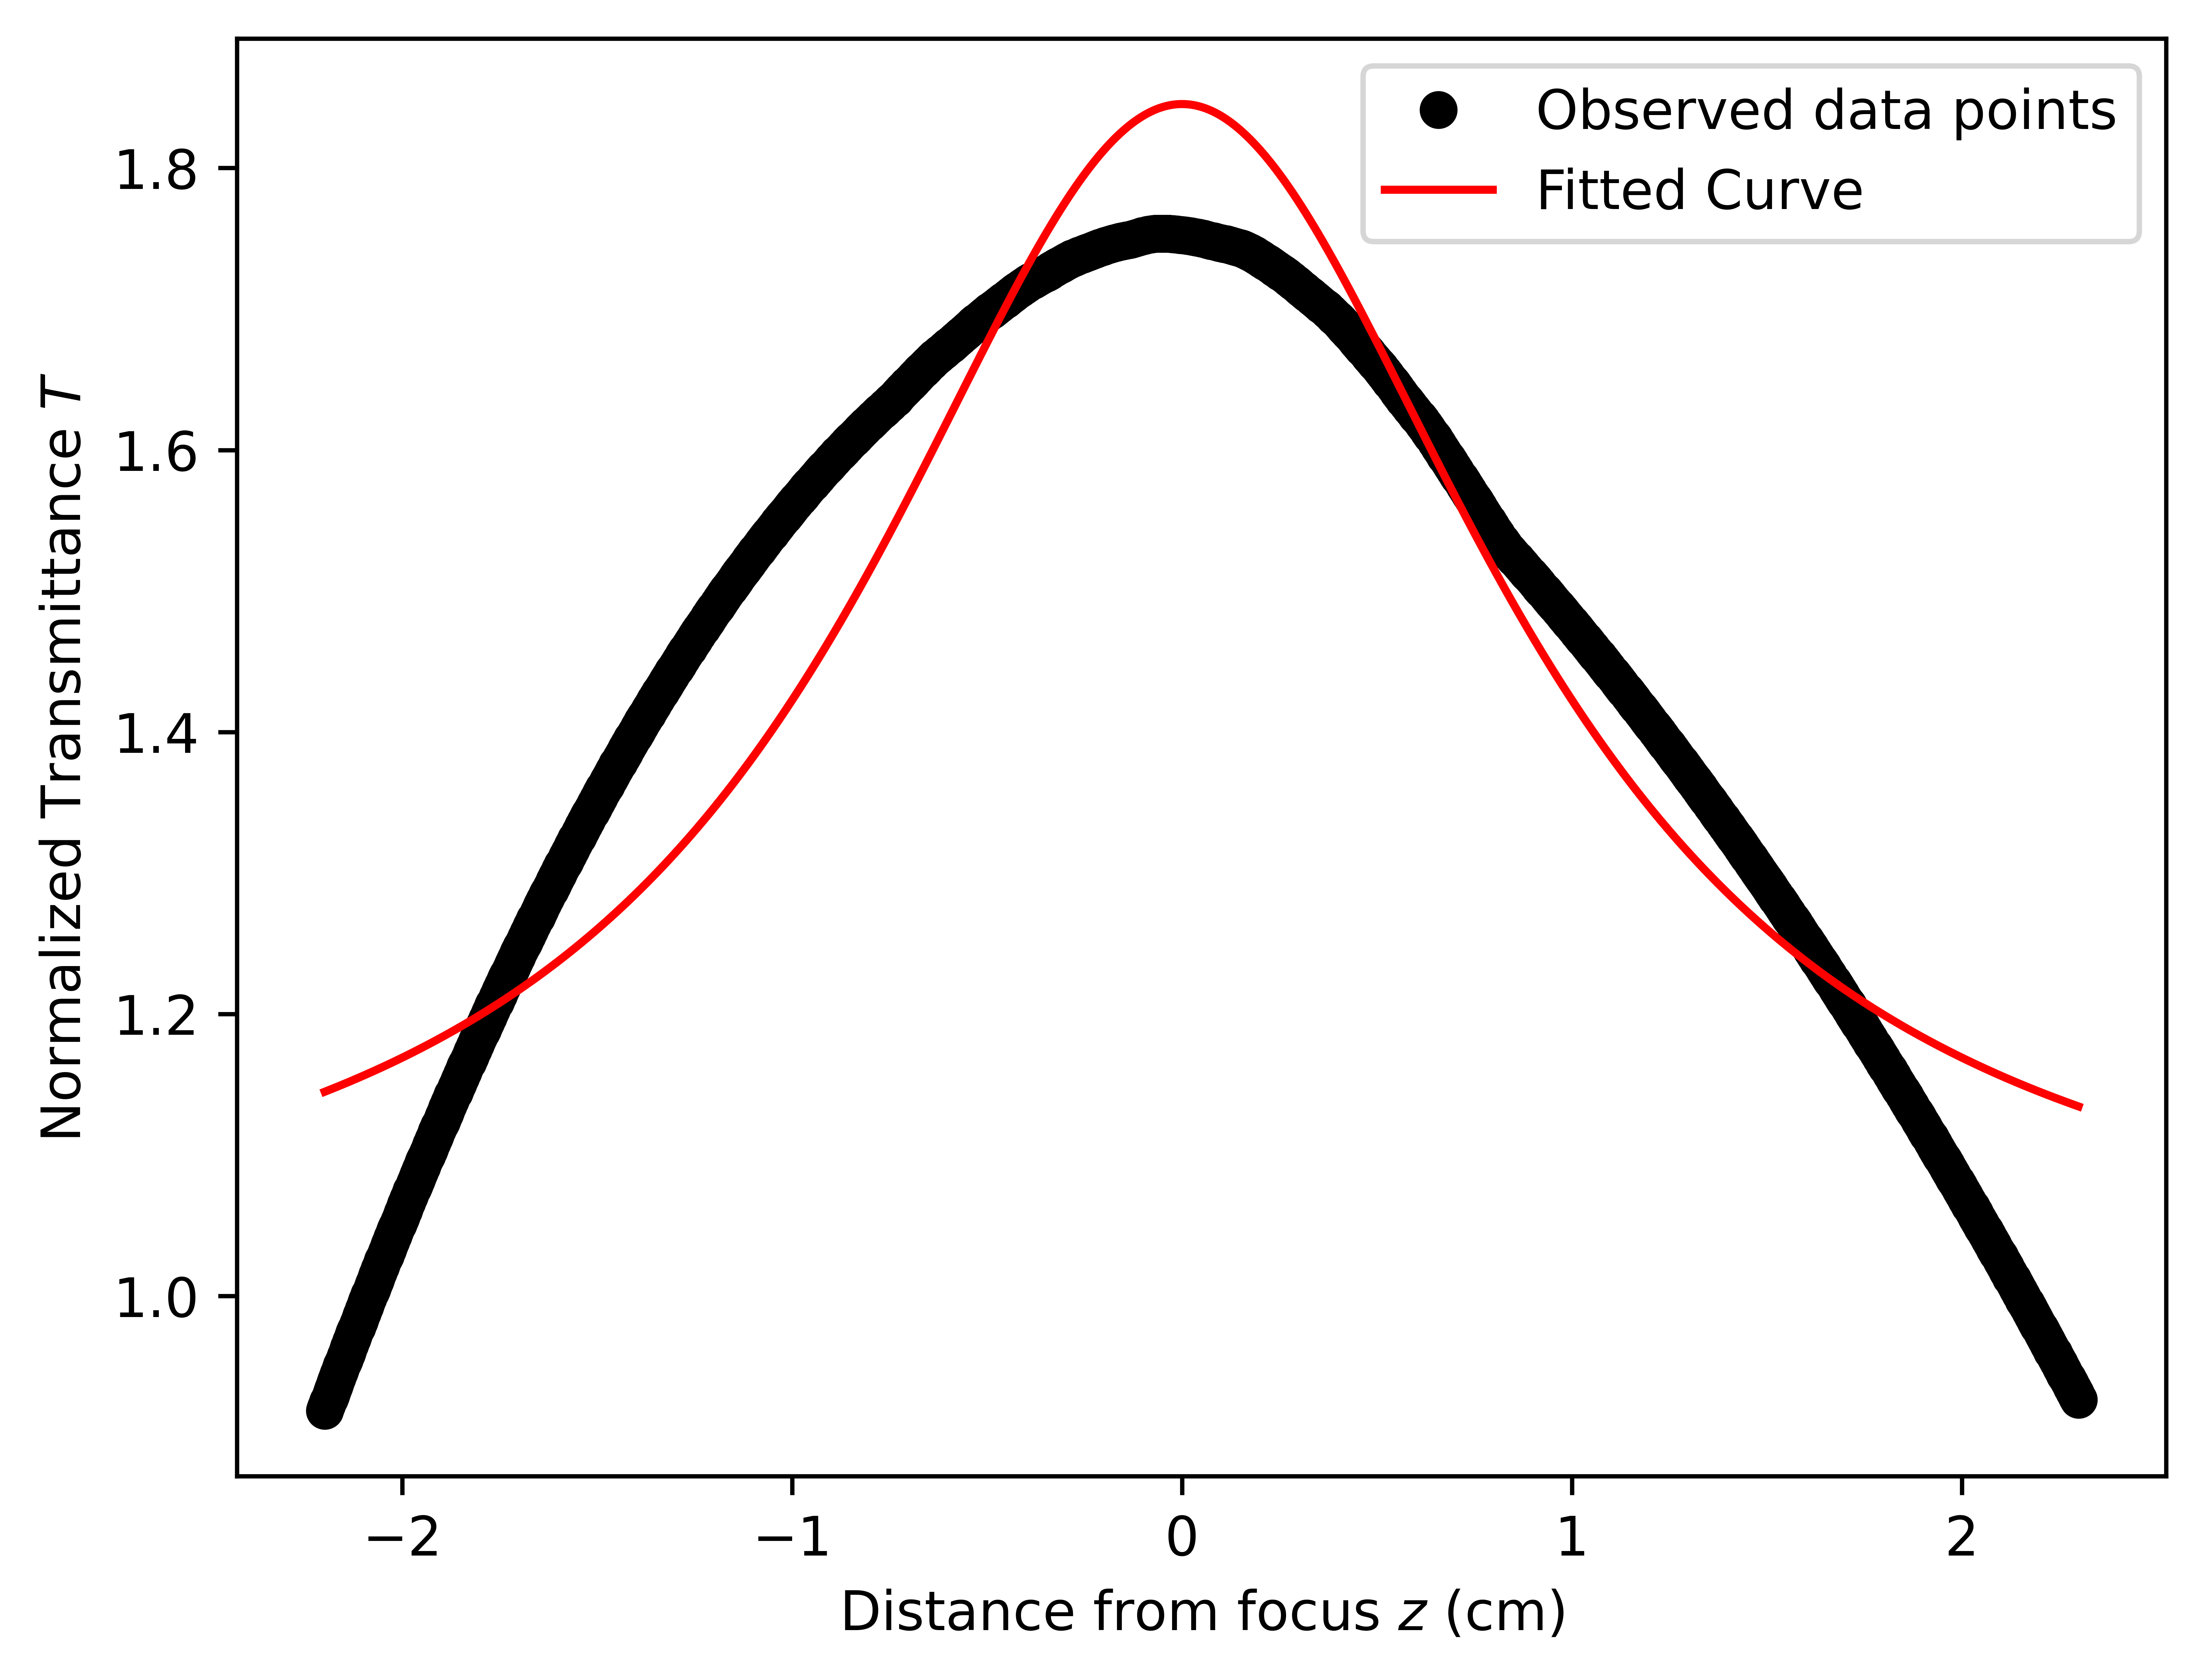
\includegraphics[scale = 0.59]{satys-o}
			\caption{Variation of transmittance with distance for methyl ammonium lead iodide thin film (open aperture)}
		\end{figure}
	
	\subsection{With methyl ammonium lead iodide solution}
		\subsubsection{Closed Aperture}
		After fitting the recorded data according to \eqref{eq:29} the following observations were made:
		\begin{enumerate} 
			\item Average power, $ \langle P \rangle  = \SI{150}{\milli \watt}$
			\item Second order non-linear refractive index, $ n_2 = \SI[separate-uncertainty=true]{-3.9 \pm 0.9e-18}{\meter \squared \per \watt} $.
		\end{enumerate}
		\begin{figure}
			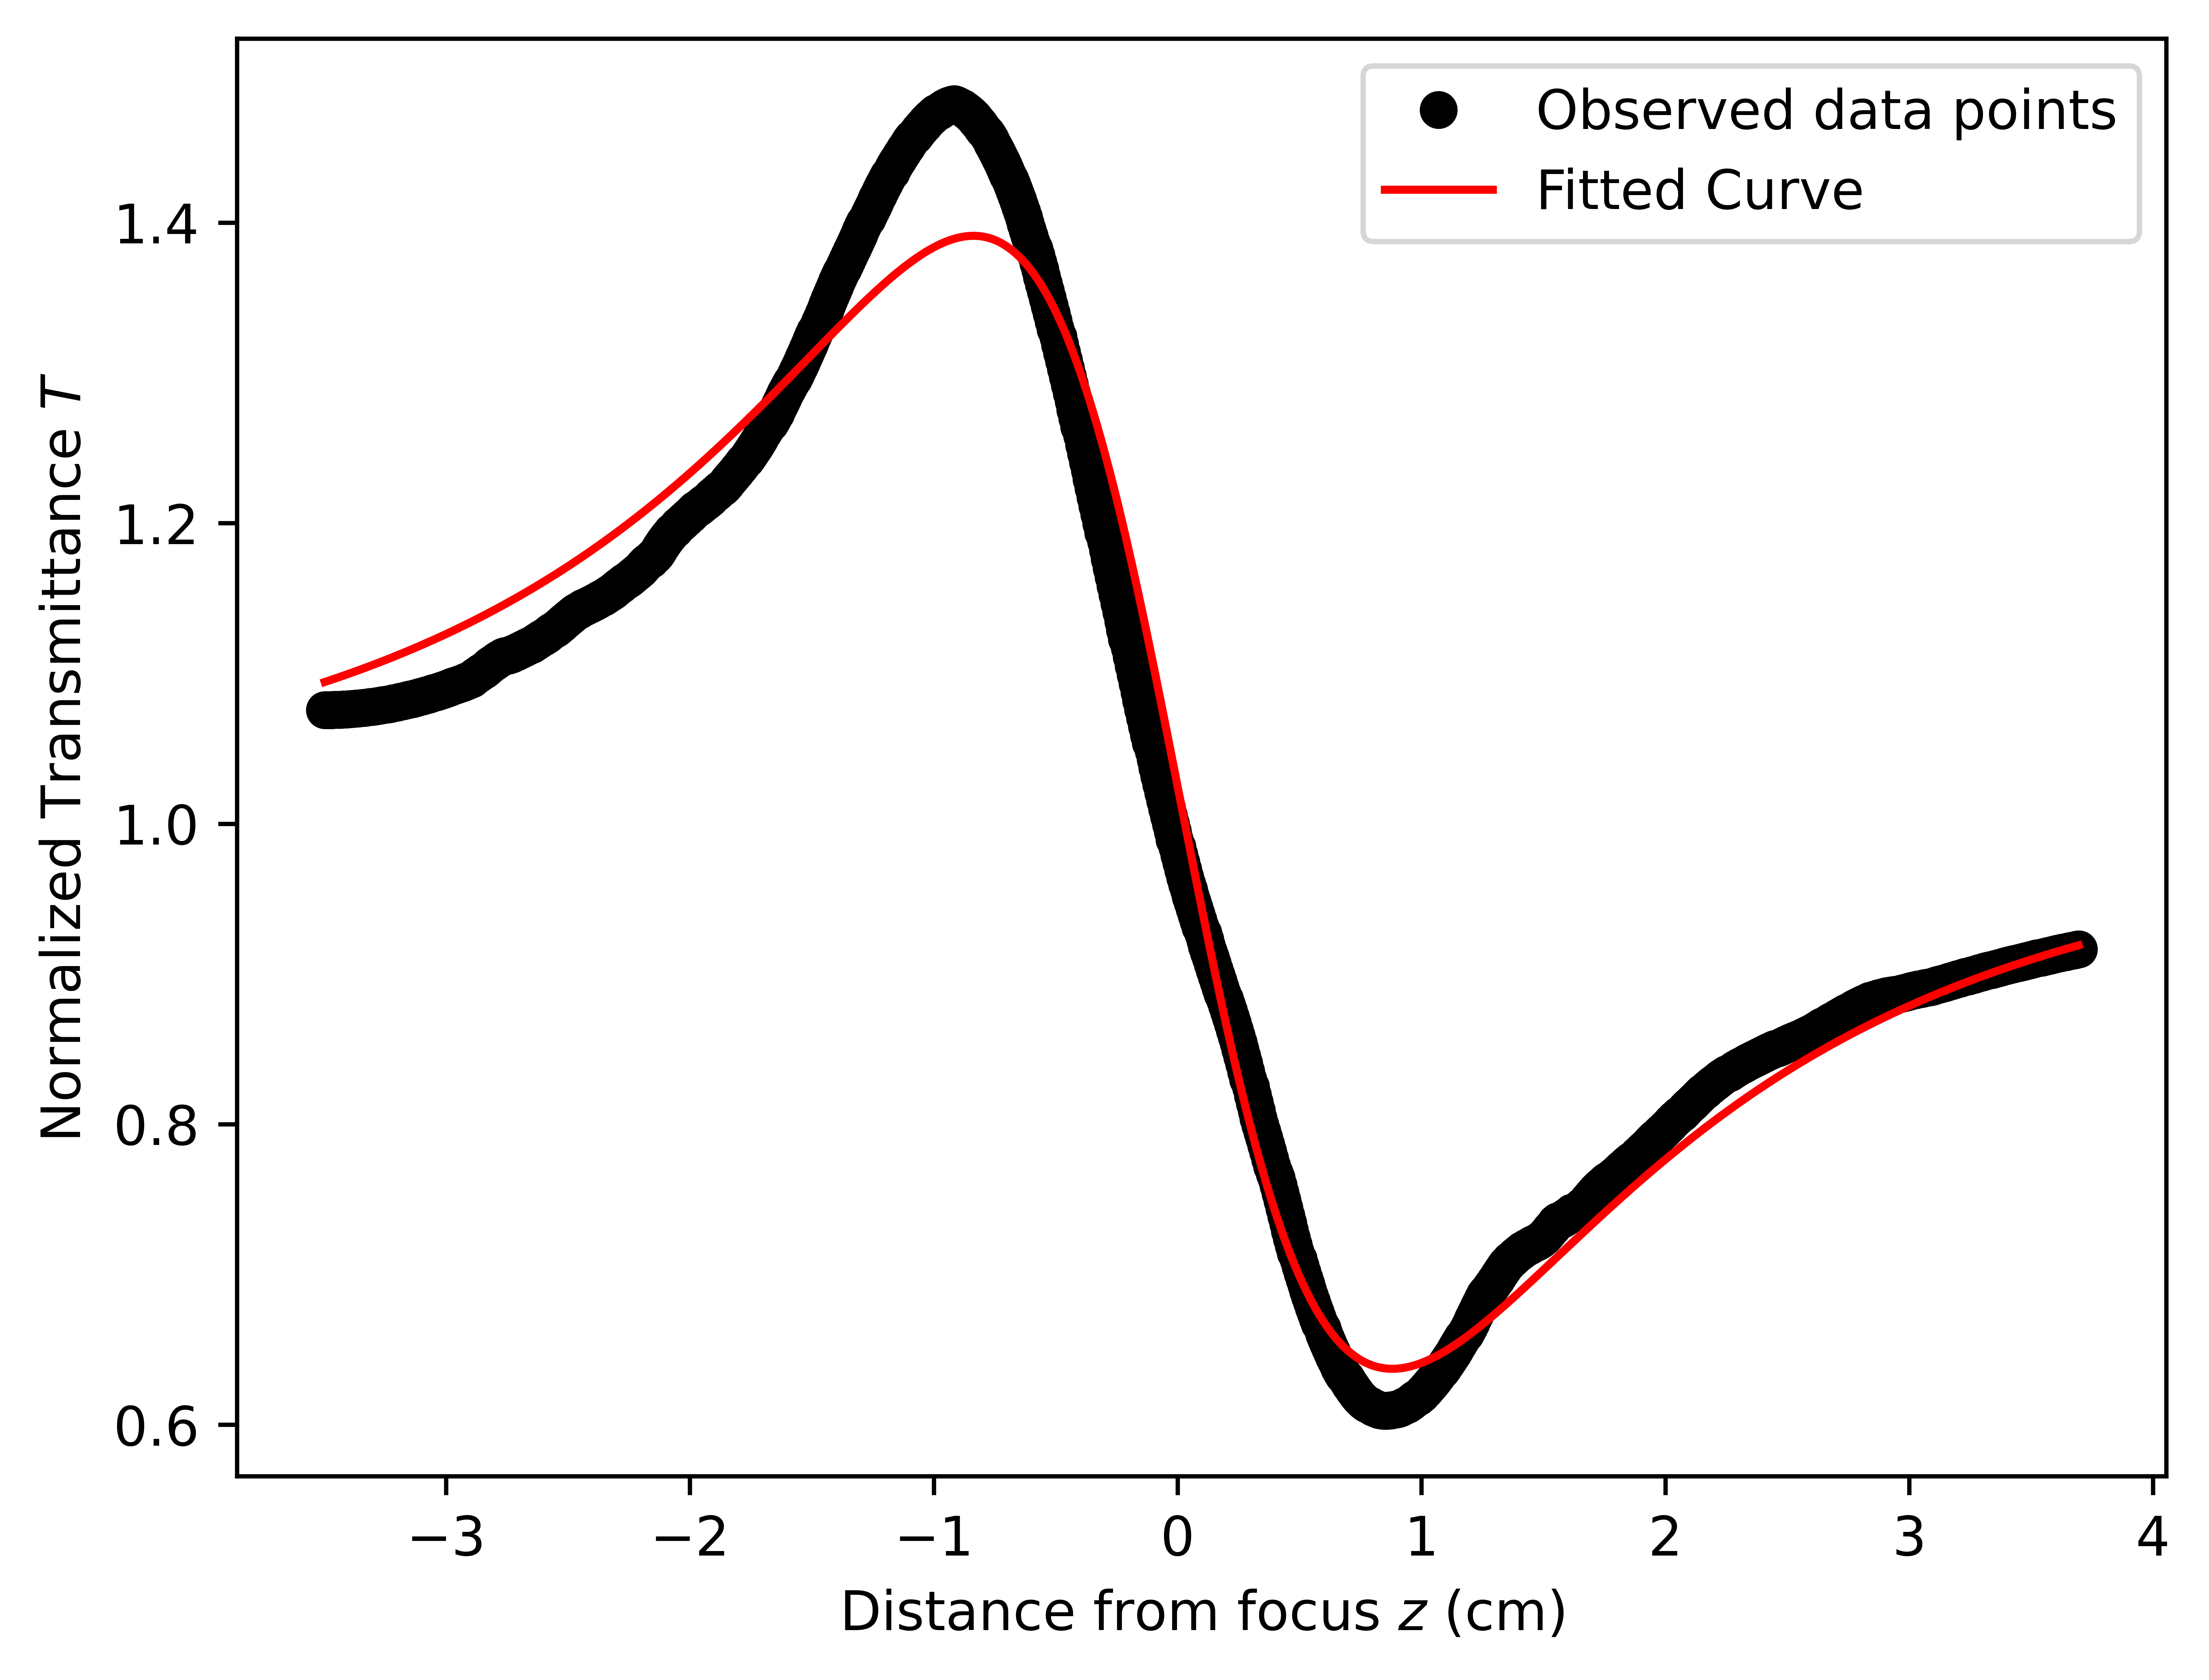
\includegraphics[scale = 0.59]{satyl-c}
			\caption{Variation of transmittance with distance for methyl ammonium lead iodide solution (closed aperture)}
		\end{figure}
		
		\subsubsection{Open Aperture}
		After fitting the recorded data according to \eqref{eq:30} the following observations were made:
		\begin{enumerate} 
			\item Average power, $ \langle P \rangle  = \SI{100}{\milli \watt}$
			\item Non-linear absorption coefficient, $ \beta = \SI[separate-uncertainty=true]{-3.2 \pm 0.7e-19}{\meter \per \watt} $.
		\end{enumerate}
		\begin{figure}
			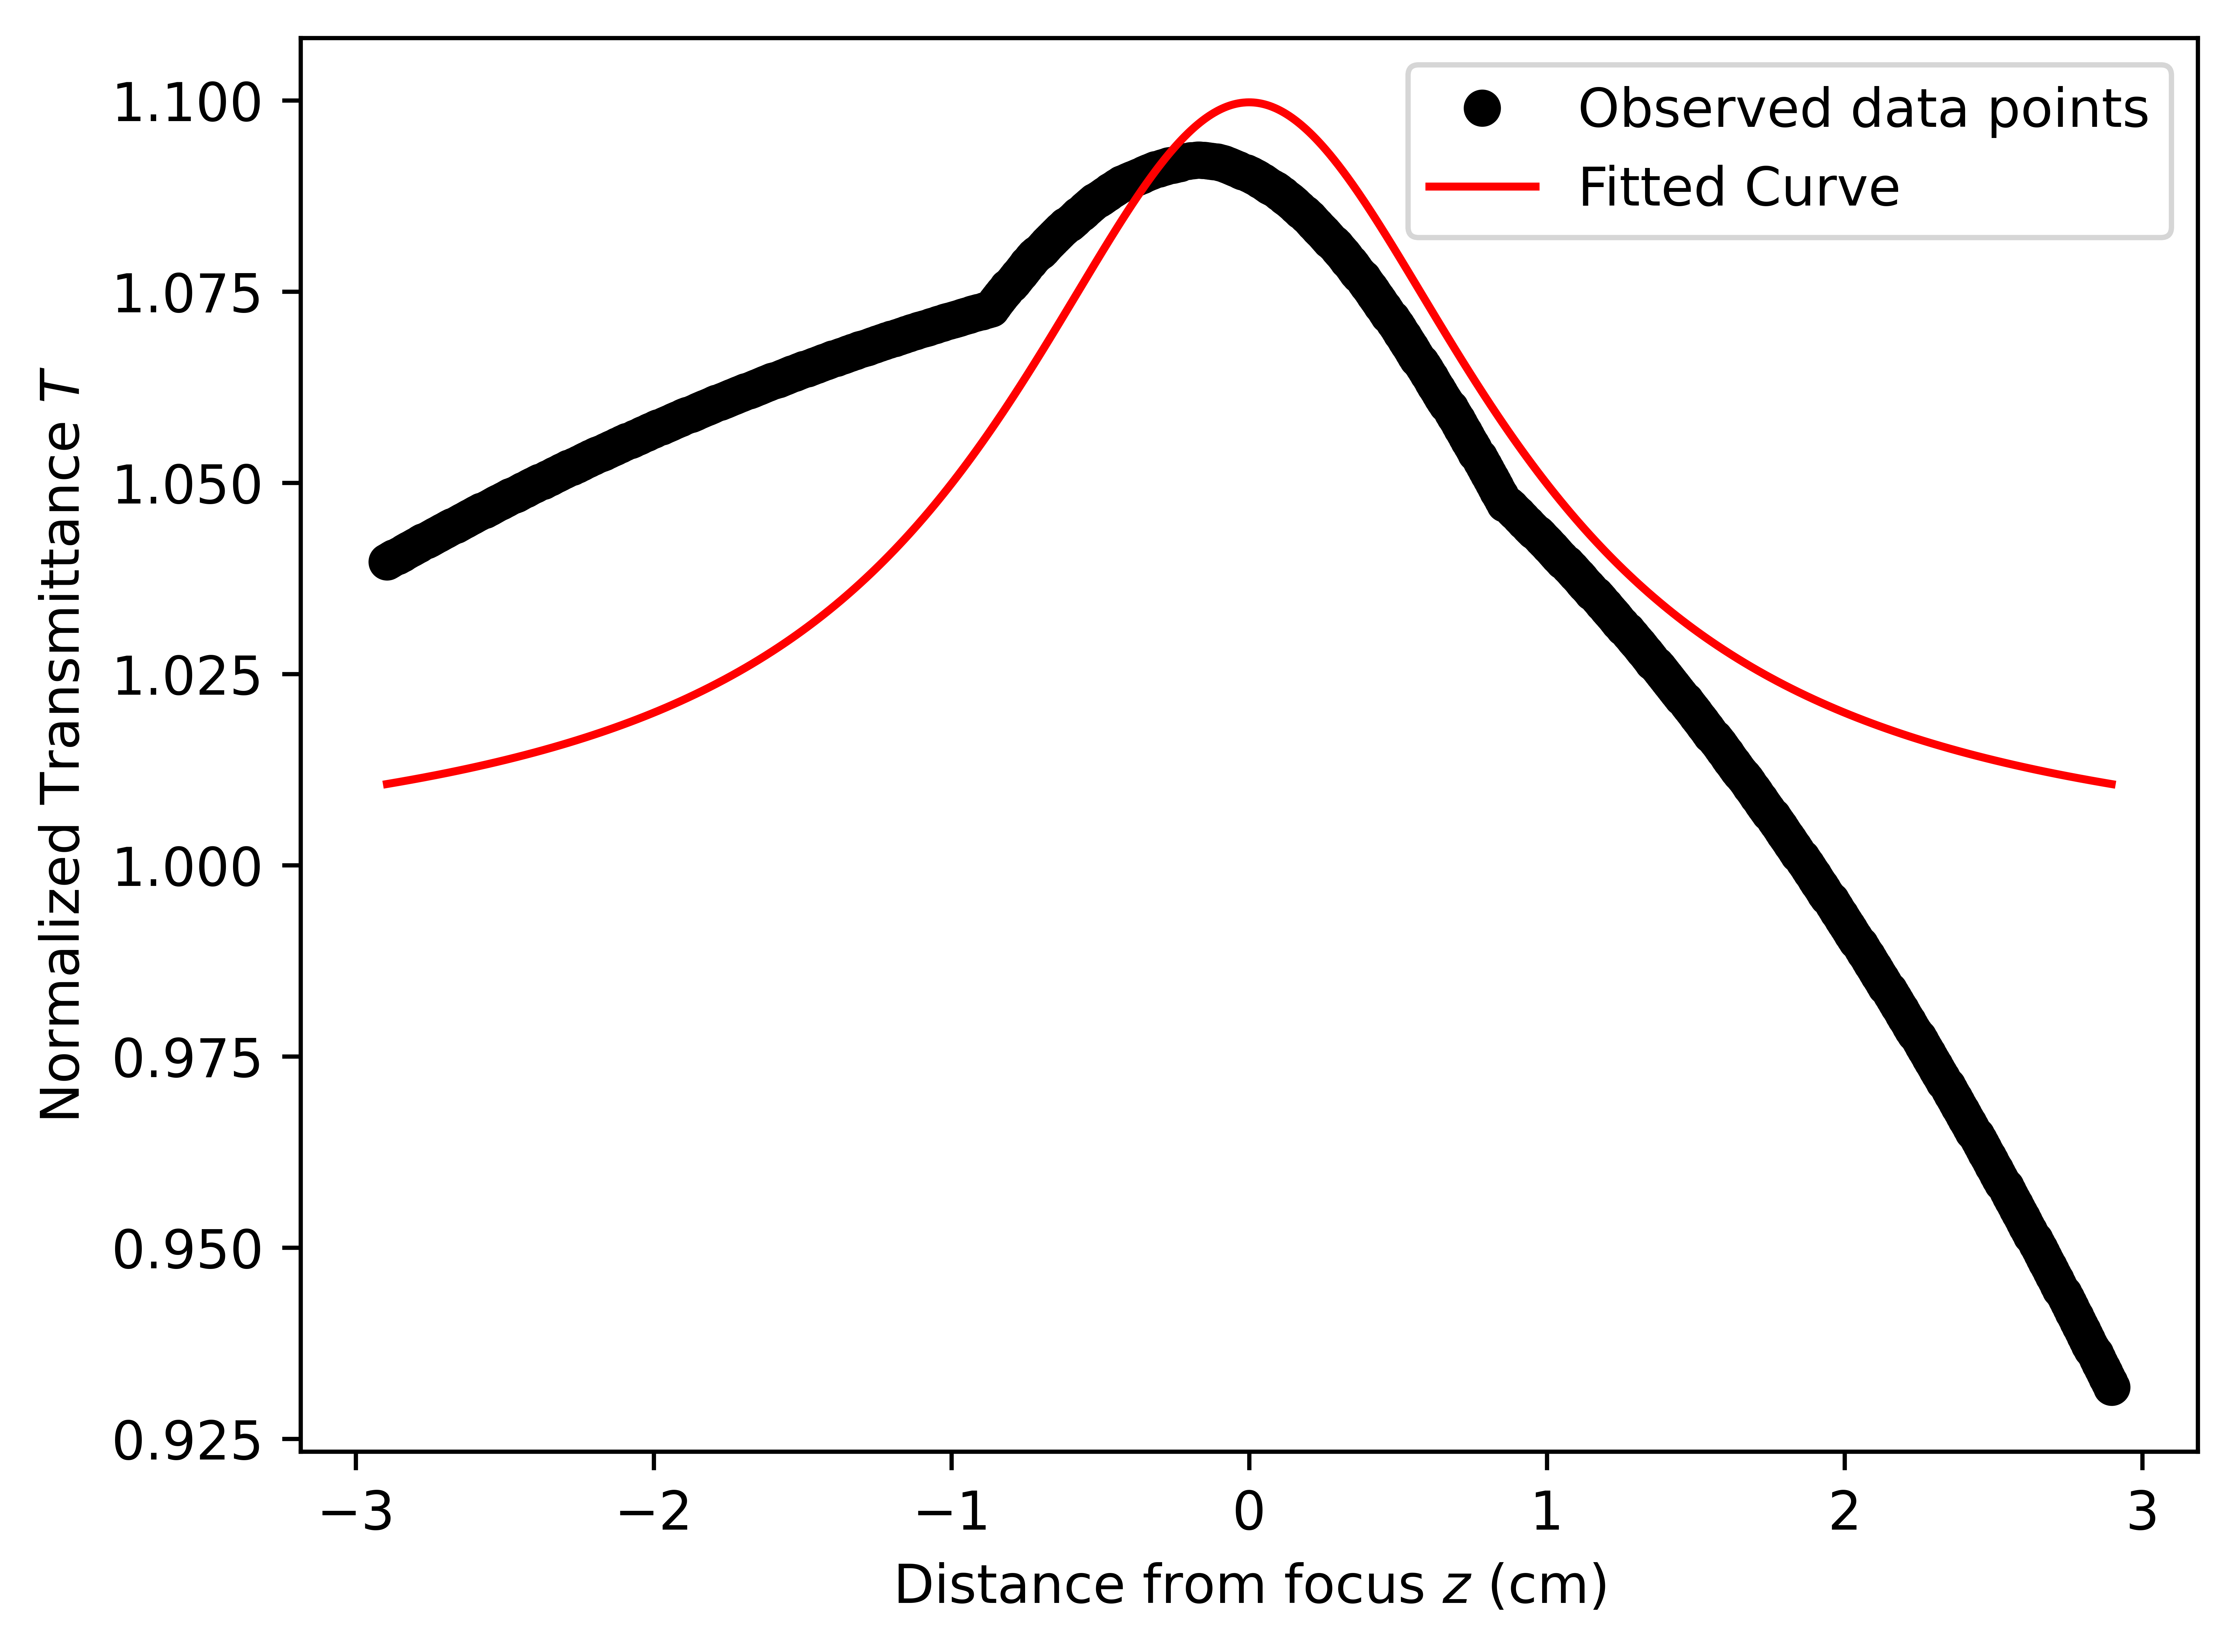
\includegraphics[scale = 0.59]{satyl-o}
			\caption{Variation of transmittance with distance for methyl ammonium lead iodide solution (open aperture)}
		\end{figure}
	
	\subsection{With an organic sample thin film}
		A solution of organics compound Bis(salicylidene)-1,2-cyclohexanediamine (Figure \ref{fig:org-s}) was also used to perform the Z-scan experiment. Using the spin-coating deposition technique a thin-film of the sample was deposited on a substrate.
		\begin{figure}\label{fig:org-s}
			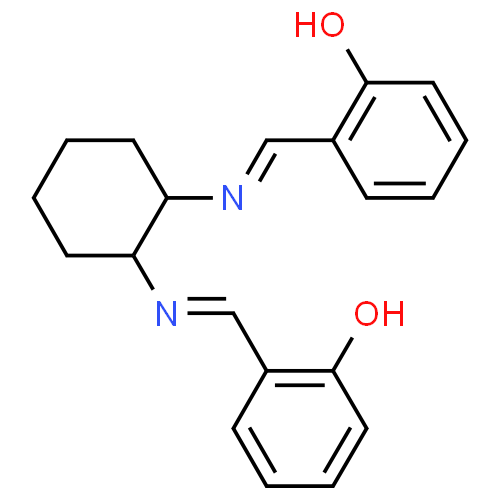
\includegraphics[scale = 0.3]{org-s}
			\caption{Bis(salicylidene)-1,2-cyclohexanediamine}
		\end{figure}
		\subsubsection{Closed Aperture}
		After fitting the recorded data according to \eqref{eq:29} the following observations were made:
		\begin{enumerate} 
			\item Average power, $ \langle P \rangle  = \SI{180}{\milli \watt}$
			\item Second order non-linear refractive index, $ n_2 = \SI[separate-uncertainty=true]{-8.1 \pm 1.8e-18}{\meter \squared \per \watt} $.
		\end{enumerate}
		\begin{figure}
			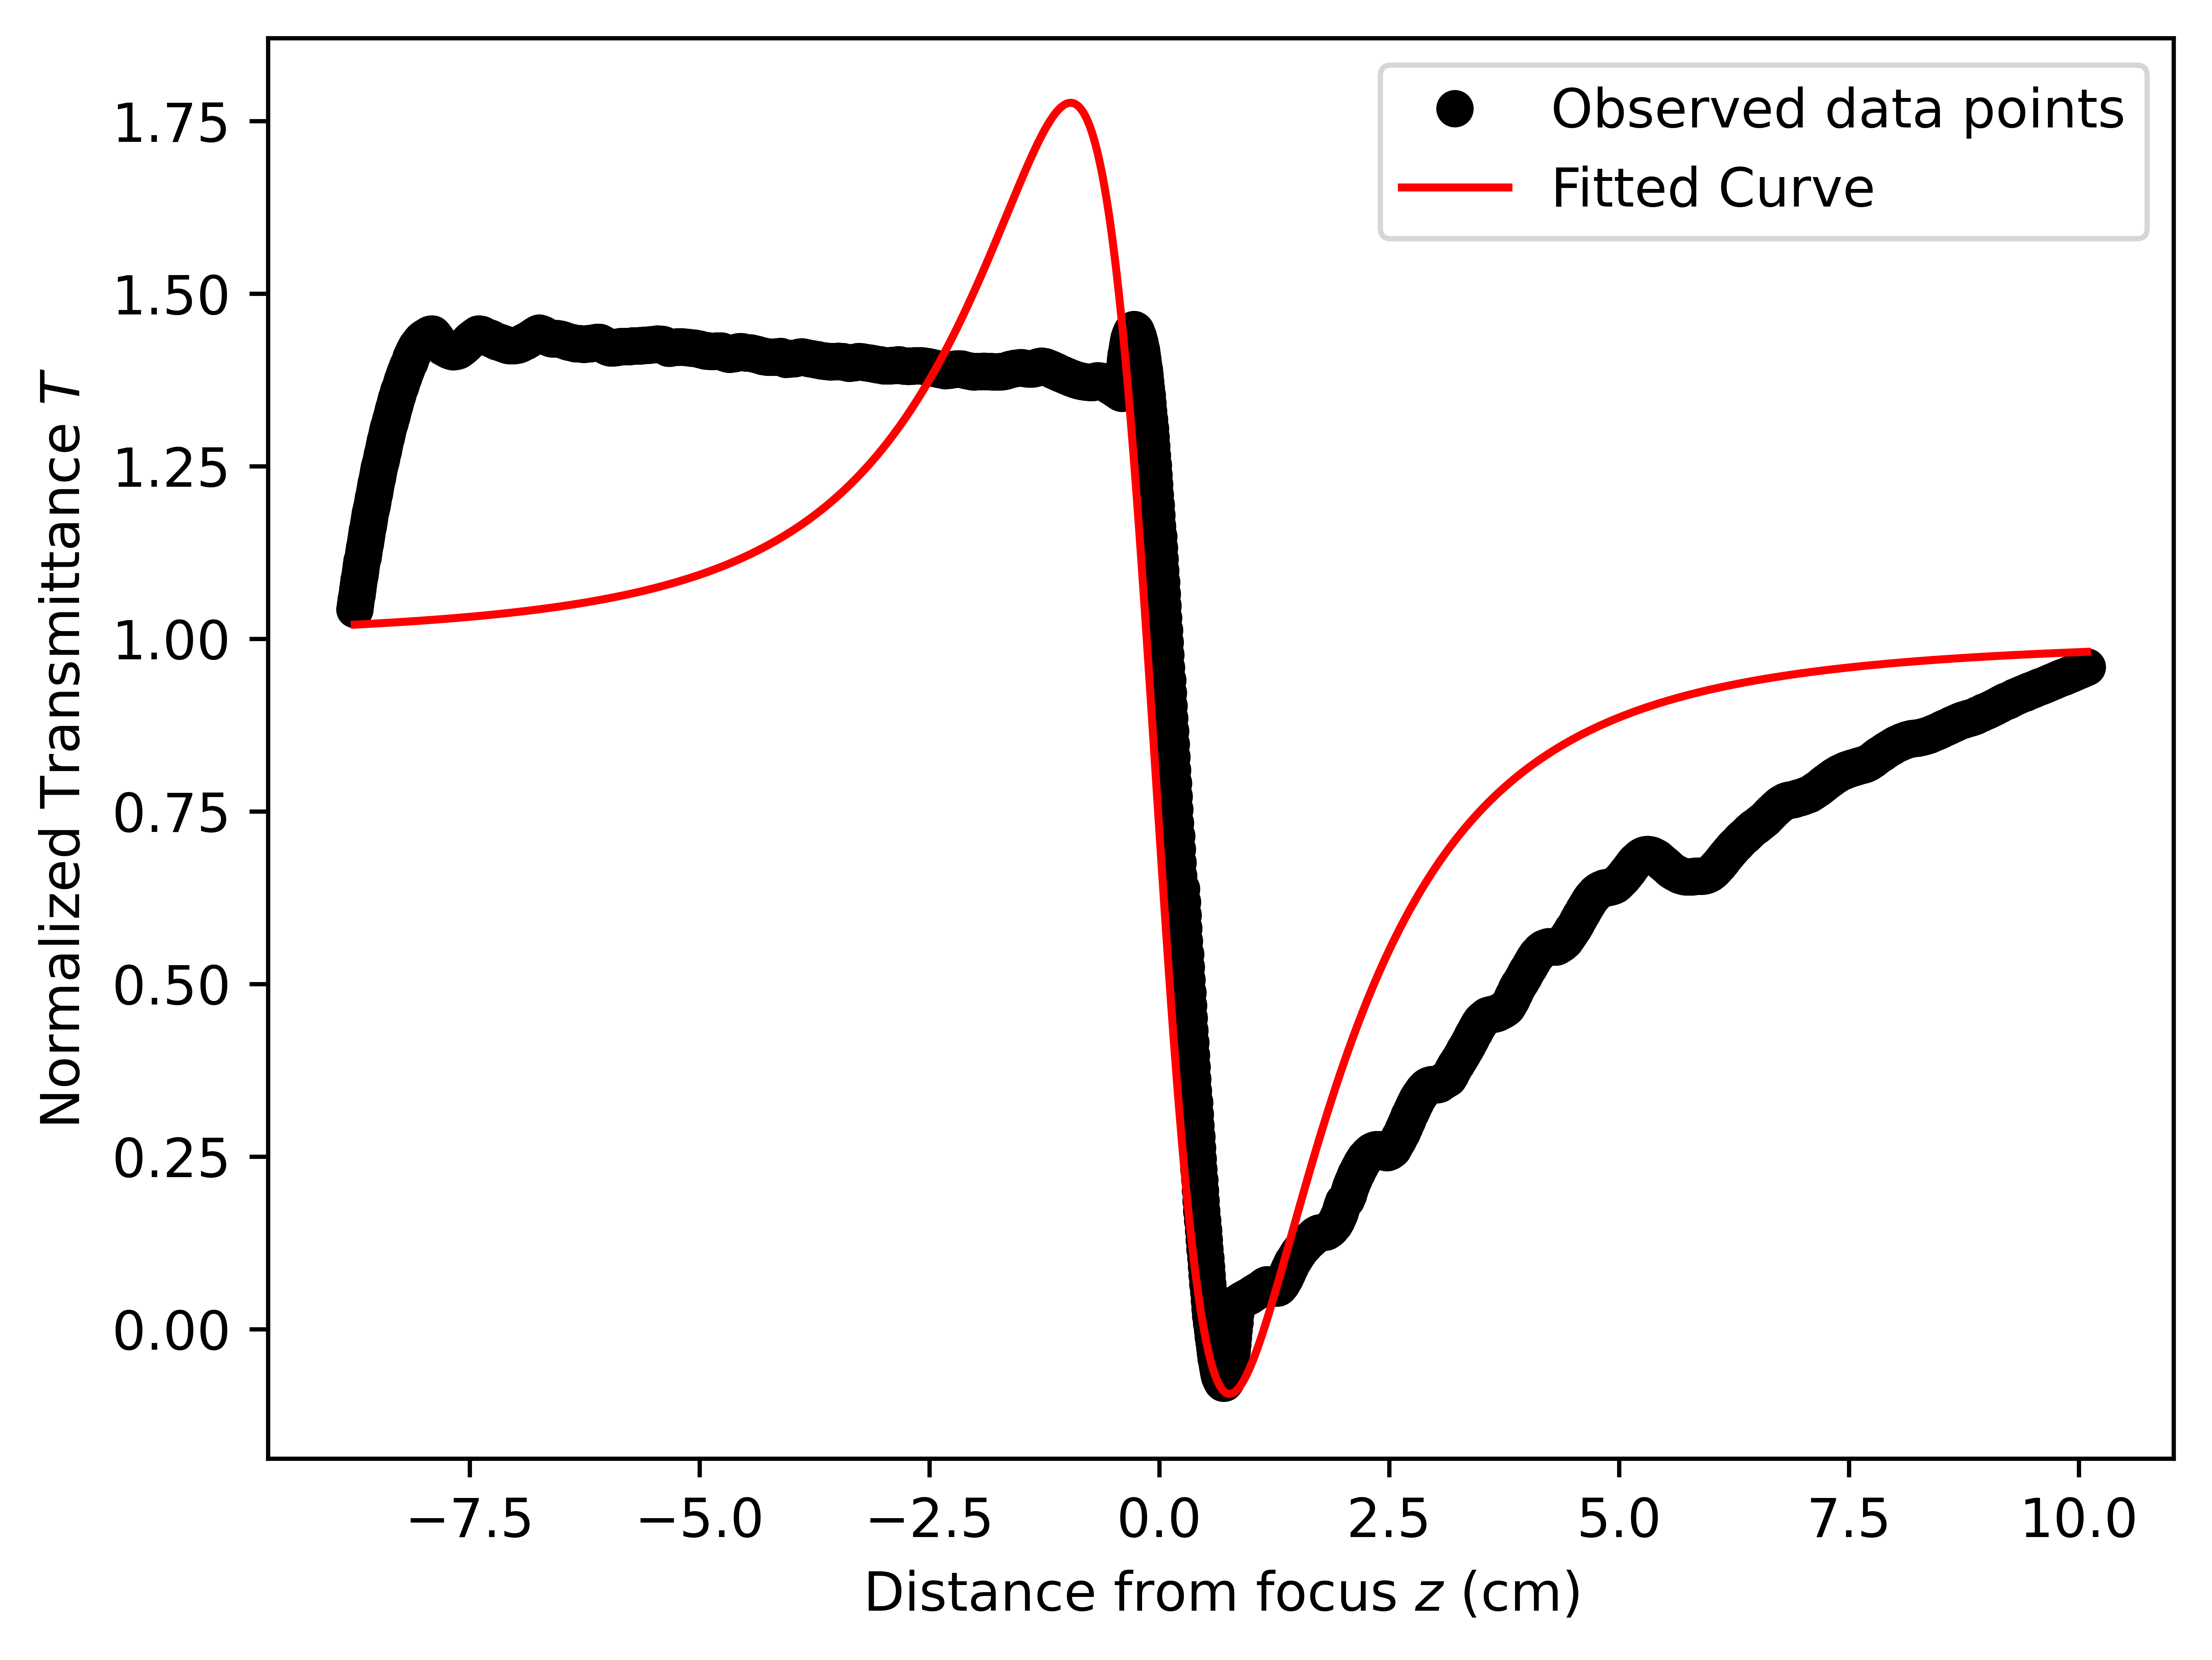
\includegraphics[scale = 0.59]{org-c}
			\caption{Variation of transmittance with distance for Bis(salicylidene)-1,2-cyclohexanediamine thin film (closed aperture)}
		\end{figure}
		
		\subsubsection{Open Aperture}
		After fitting the recorded data according to \eqref{eq:30} the following observations were made:
		\begin{enumerate} 
			\item Average power, $ \langle P \rangle  = \SI{25}{\milli \watt}$
			\item Non-linear absorption coefficient, $ \beta = \SI[separate-uncertainty=true]{8.5 \pm 1.9e-19}{\meter \per \watt} $.
		\end{enumerate}
		\begin{figure}
			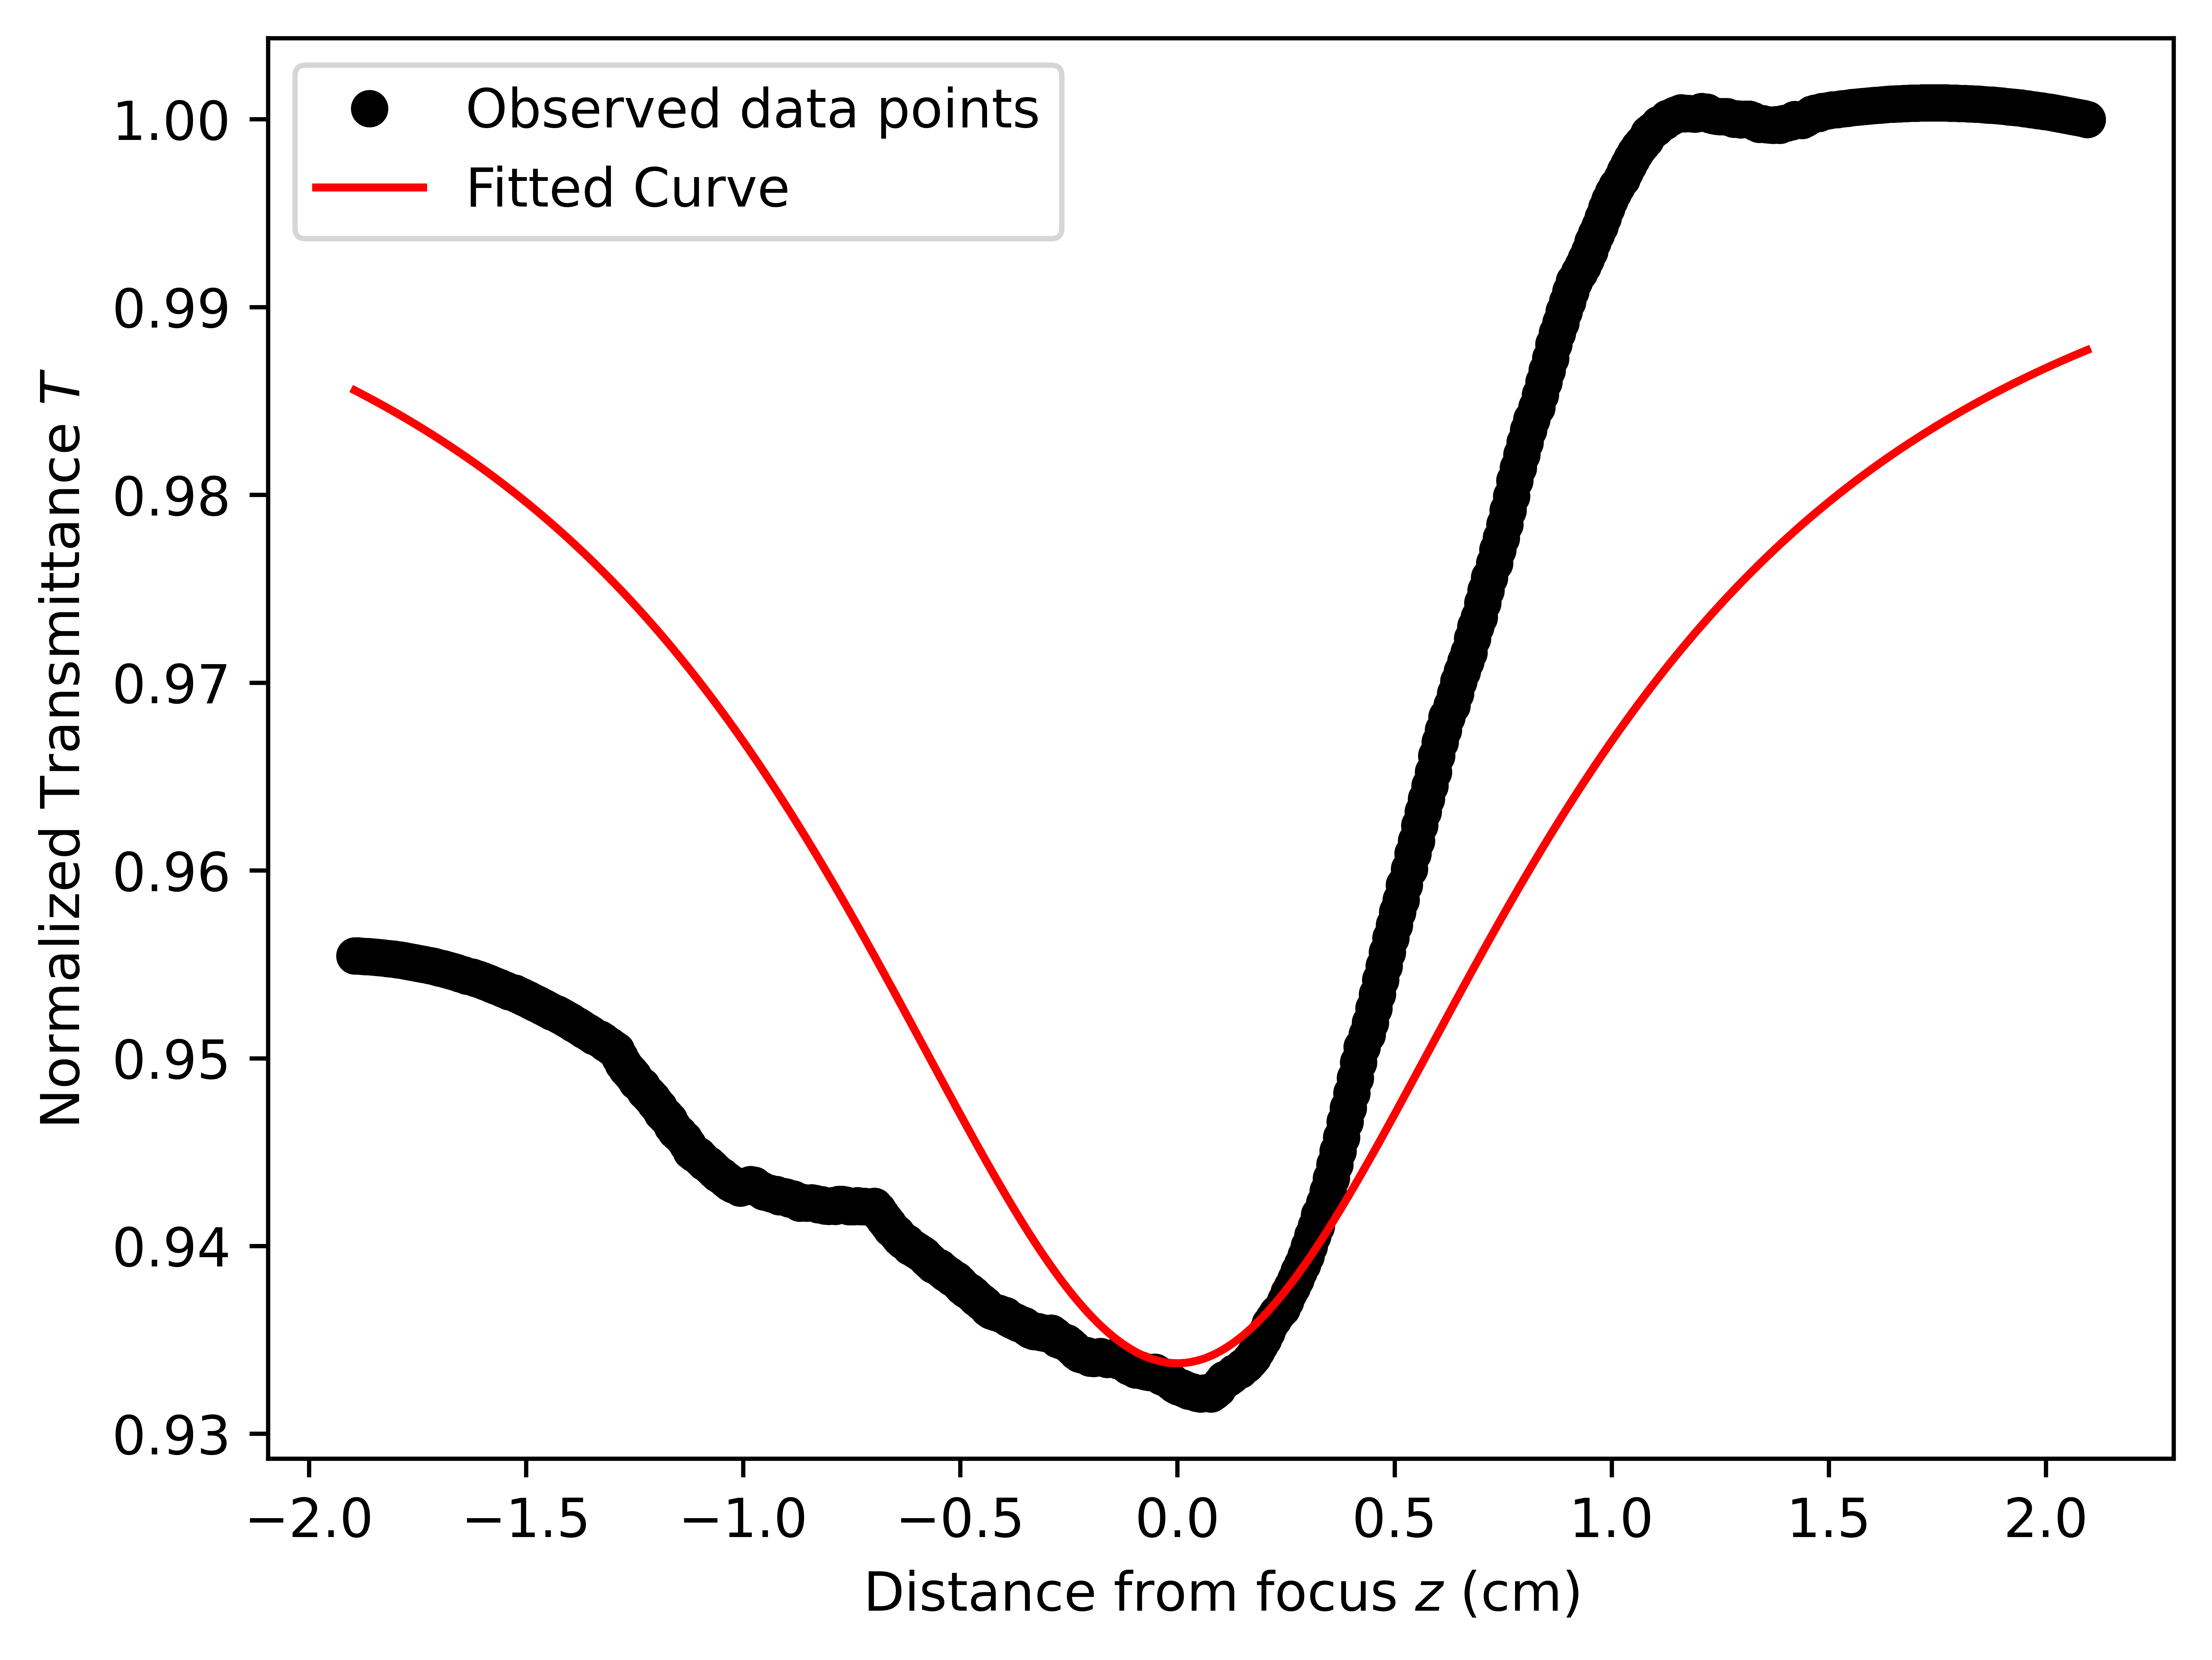
\includegraphics[scale = 0.59]{org-o}
			\caption{Variation of transmittance with distance for Bis(salicylidene)-1,2-cyclohexanediamine thin film (open aperture)}
		\end{figure}
		
\section{Discussions}
	\begin{enumerate}
		\item While taking observations, we noticed that there were
		some places near the focus where we found some sudden fluctuations in transmittance. To remove the dip, we
		tried reducing the power. The magnitude of the fluctuations was somewhat minimized but they could not be removed completely. 
		\item During data analysis, we employed Python's SciPy package and used its subroutine to remove the fluctuations (based on the Savitzky–Golay filter) for a better fit to the our theoretical model. 
		\item In the case of the organic sample in thin film form, there were multiple dips after the focus resulting in sub-par data. In case of solution of the same sample, the data obtained was not presentable due
		to too much dominance of the multiple interference
		fluctuations. 
		\item This may be due to high absorption coefficient
		for the sample so that the refractive index changes
		very rapidly due to significant thermal variation along
		\item We performed the experiment for the same sample and verified that the refractive index and absorption coefficient were within the margin of error. The discrepancies could be explained by the relative instability of the cuvette when performing the experiment with solution.
	\end{enumerate}
	
	
\section{Conclusions}
	\begin{enumerate}
		\item We can use Z-scan experimental configuration to obtain nonlinear refractive
		index and nonlinear absorption coefficients of any standard samples. 
		\item The
		sign and magnitude of nonlinear refractive index of the samples can measured. 
		\item Using the equations of normalized transmittance and fitting
		them with the data points and will report the refractive index and nonlinear
		absorption coefficients.
		\item The property of non-linear sample to change refractive index on changing intensity can be used to make a optical transistor
		type of thing.
	\end{enumerate}

\section{Precautions and sources of error}
	\begin{enumerate}
		\item The polariser should be used to reduce the power of the laser in order
		to reduce the thermal effects of laser on the samples.
		\item Protective glasses must be worn while taking measurements and the
		laser beam shouldn’t allowed to fall outside here and there by carefully
		blocking it with black aluminium plate.
		\item The lasers should be turned off when not in use.
		\item Make sure that the temperature is below $ 23 \degree $ C
		while turning on the Laser. Else, switch it off.
		\item Make sure you keep the Laser at low power($ \sim 40 \% $) while doing alignment.
		\item Make sure to align each optical component correctly by avoiding back reflections.
		\item Make sure that the power on the main arm of the
		setup is small so as the sample does not overheat
		and lose its properties.
	\end{enumerate}
	
	
	
\appendix
\section{Pulsed lasers}\label{pulsed}
	In this laser, we used a pulsed laser which refers to any laser not classified as continuous wave, so that the optical power appears in pulses of some duration at some repetition rate.
	\par 
	Since the pulse energy is equal to the average power divided by the repetition rate, this goal can sometimes be satisfied by lowering the rate of pulses so that more energy can be built up in between pulses. In laser ablation for example, a small volume of material at the surface of a work piece can be evaporated if it is heated in a very short time, whereas supplying the energy gradually would allow for the heat to be absorbed into the bulk of the piece, never attaining a sufficiently high temperature at a particular point.
	\subsection{Q-switching}
		In a Q-switched laser, the population inversion is allowed to build up by introducing loss inside the resonator which exceeds the gain of the medium; this can also be described as a reduction of the quality factor or 'Q' of the cavity. Then, after the pump energy stored in the laser medium has approached the maximum possible level, the introduced loss mechanism (often an electro- or acousto-optical element) is rapidly removed (or that occurs by itself in a passive device), allowing lasing to begin which rapidly obtains the stored energy in the gain medium. This results in a short pulse incorporating that energy, and thus a high peak power.
	\begin{figure}
		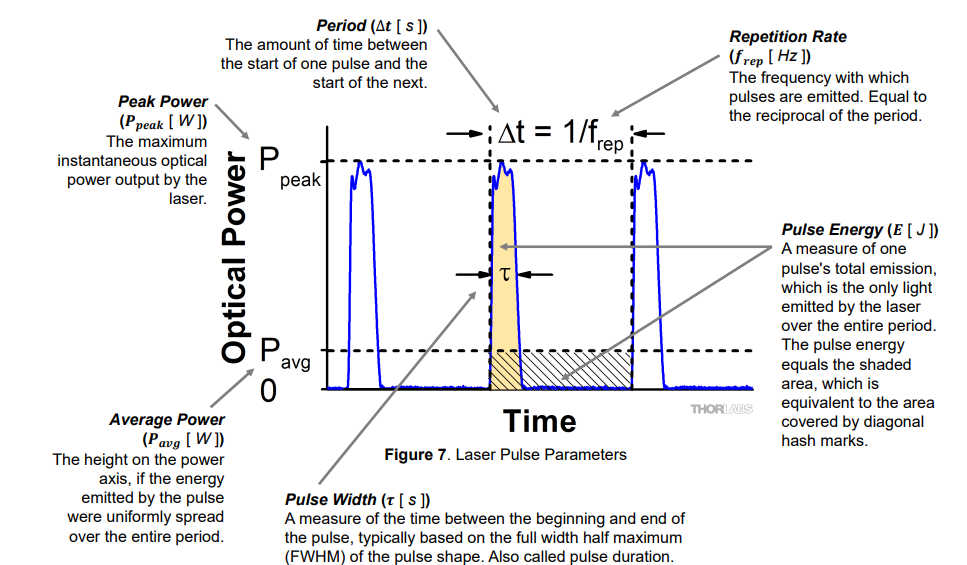
\includegraphics[scale = 0.41]{pulsedlaser}
		\caption{Terminology related to a pulsed laser}
	\end{figure}
\section{Spin-coating}
	A thin film is a layer of material ranging from fractions of a nanometer (monolayer) to several micrometers in thickness. The controlled synthesis of materials as thin films (a process referred to as deposition) is a fundamental step in many applications.
	\par 
	The act of applying a thin film to a surface is thin-film deposition – any technique for depositing a thin film of material onto a substrate or onto previously deposited layers. We employed the use of a deposition technique called \textit{spin coating}.
	\par 
	Spin coating is a procedure used to deposit uniform thin films onto flat substrates. Usually a small amount of coating material is applied on the center of the substrate, which is either spinning at low speed or not spinning at all. The substrate is then rotated at speed up to 10,000 rpm to spread the coating material by centrifugal force. A machine used for spin coating is called a spin coater, or simply spinner. Spin coating is widely used in microfabrication of functional oxide layers on glass or single crystal substrates using sol-gel precursors, where it can be used to create uniform thin films with nanoscale thicknesses.
	\par 
	The methyl ammonium lead iodide thin film was prepared this way in the Nanoelectronics lab.
% The \nocite command causes all entries in a bibliography to be printed out
% whether or not they are actually referenced in the text. This is appropriate
% for the sample file to show the different styles of references, but authors
% most likely will not want to use it.
\nocite{*}

\bibliography{apssamp}% Produces the bibliography via BibTeX.

\end{document}
%
% ****** End of file apssamp.tex ******
